\documentclass[a4paper,10pt]{book}
\usepackage[utf8]{inputenc}
\usepackage{graphicx}
\usepackage{amsmath}
\usepackage{amsfonts}
\usepackage{url}
\usepackage[rmargin=1cm, lmargin=1cm]{geometry}

\newcommand{\sen}{\operatorname{sen}\,}
\newcommand{\senh}{\operatorname{senh}\,}
\renewcommand{\sin}{\operatorname{sen}\,}
\renewcommand{\sinh}{\operatorname{senh}\,}


\begin{document}

\chapter{16 de outubro}
\section{Funções periódicas}

Uma função $f:\mathbb{R}\to \mathbb{R}$ (ou $f:\mathbb{R}\to \mathbb{C}$ ) é dita periódica se existe $T>0$ tal que:
$$f(t+T)=f(t),~~ \forall t\in \mathbb{R}.$$

Aqui $T$ é chamado período e a função é dita $T$-periódica.

{\bf Exemplos:} Você conhece? $\cos(t), \sin(t)$.

% 
{\bf Observação:} Se $f(t)$ é $T$-periódica, $\alpha f(t)$ também é.

{\bf Observação:} Se $T$ é período de uma função $f(t)$ então todo múltiplo inteiro de $T$ também é período:
 $$f(t+nT)=f(t).$$
% 

{\bf Perguntas:} A soma de funções periódicas é periódica?

{\bf Resposta:} Se $f(t)$ tem período $T_1$ e g(t) tem período $T_2$ e $\frac{T_1}{T_2}=\frac{n}{m}$, isto é, $mT_1 = nT_2$, então $f(t)+g(t)$ é periódica. Aqui $n$ e $m$ são inteiros positivos.
{\bf Dem:} Construtiva com $T=mT_1$:
$$f(t+T)+g(t+T)=f(t+nT_1)+g(t+mT_2)=f(t)+g(t)$$
% 

 {\bf Definição:} Se $f(t)$ é periódica e existe $T_f$ o menor período, então $T_f$ é chamado de período fundamental e $w_f:=\frac{2\pi}{T_f}$ é a frequência angular fundamental.

{\bf Pergunta:} Existem funções periódicas sem período fundamental?
$$f(t)=1$$
% 
\subsection{Polinômios trigonométricos e séries trigonométricas}
 Seja $T>0$, definimos polinômio trigonomético de grau $N$ uma função do tipo:
 \begin{equation}f(t)=\frac{a_0}{2}+ \sum_{n=1}^N \left[a_n \cos(w_n t) + b_n \sen(w_nt)\right] \end{equation}
 onde $w_n=\frac{2\pi n}{T}$.
% 

  Seja $T>0$, definimos série trigonométrica toda função do tipo:
\begin{equation}f(t)=\frac{a_0}{2}+ \sum_{n=1}^\infty \left[a_n \cos(w_n t) + b_n \sen(w_n t)\right] \end{equation}
 onde $w_n=\frac{2\pi n}{T}$.


 {\bf Exemplo:}
  Mostre que $T$ é um período para séries e  polinômios trigonométricos acima definidos.

 \subsection{Relações de ortogonalidade}
 \begin{eqnarray*}
 \int_{0}^T \sen\left(\frac{2\pi nt}{T}\right) \sen\left(\frac{2\pi mt}{T}\right)dt&=&\left\{
 \begin{array}{ll}0, &n\neq m\\ \frac{T}{2}, &n=m\neq 0 \end{array} \right.\label{rel_ort_ss}\\
 \int_{0}^T \cos\left(\frac{2\pi nt}{T}\right) \cos\left(\frac{2\pi mt}{T}\right)dt&=&\left\{
 \begin{array}{ll}0, &n\neq m\\ \frac{T}{2}, &n=m\neq 0\\ T,&n=m=0 \end{array} \right.\label{rel_ort_cc}\\
 \int_{0}^T \cos\left(\frac{2\pi nt}{T}\right) \sen\left(\frac{2\pi mt}{T}\right)dt&=&0\label{rel_ort_sc}\label{rel_ort_cs}
 \end{eqnarray*}

\subsection{Forma harmônica}
$$A\cos(wt-\phi)=A\left[\cos(wt)\cos(\phi)+\sin(wt)\sin(\phi)\right]$$

$$A\cos(wt-\phi)=A\cos(wt)\cos(\phi)+A\sin(wt)\sin(\phi)$$

$$A_n\cos(w_nt-\phi_n)=\underbrace{A\cos(\phi_n)}_{a_n}\cos(w_nt)+\underbrace{A\sin(\phi_n)}_{b_n}\sin(w_nt)$$

$$f(t)=A_0+\sum_{n=1}^\infty A_n\cos(w_nt-\phi_n)$$

{\bf Obs:} Para qualquer par $a_n$ e $b_n$, existem $A_n$ e $\phi_n$ que satisfazem a identidade e $A_n>0,~~\forall n>0$.

\subsection{Forma complexa ou exponencial}
\section{Forma exponencial}
A forma exponencial de uma série de Fourier é obtida quando se substiuem as funções trigonométricas $\sen(w_nt)$ e $\cos(w_nt)$ por suas representações em termos de exponenciais complexos, isto é
\begin{equation}\cos(w_nt)=\frac{e^{iw_nt}+ e^{-iw_nt}}{2}~~~\hbox{e}~~~\sen(w_nt)=\frac{e^{iw_nt}- e^{-iw_nt}}{2i}\end{equation}
\begin{eqnarray*}
f(t)&=&\frac{a_0}{2}+\sum_{n=1}^\infty a_n\cos(w_n t)+\sum_{n=1}^\infty b_n\sen(w_n t)\\
&=&\frac{a_0}{2}+\sum_{n=1}^\infty a_n\left(\frac{e^{iw_nt}+ e^{-iw_nt}}{2}\right)+\sum_{n=1}^\infty b_n\left(\frac{e^{iw_nt}- e^{-iw_nt}}{2i}\right)\\
\end{eqnarray*}
Reagrupando os termos e usando o fato que $\frac{1}{i}=-i$, temos:
\begin{eqnarray}\label{form_exp_1}
f(t)=\frac{a_0}{2}+\sum_{n=1}^\infty \frac{a_n-ib_n}{2}e^{iw_nt}+\sum_{n=1}^\infty \frac{a_n+ib_n}{2}e^{-iw_nt}
\end{eqnarray}
Agora observamos que as definições \ref{coef} dadas por  
\begin{eqnarray*}
   a_0&=& \frac{2}{T}\int_0^T f(t)dt = \frac{2}{T}\int_{-T/2}^{T/2} f(t)dt\\
   a_n&=& \frac{2}{T}\int_0^T f(t)\cos(w_n t)dt = \frac{2}{T}\int_{-T/2}^{T/2} f(t)\cos(w_nt)dt\\
   b_n&=& \frac{2}{T}\int_0^T f(t)\sen(w_n t)dt = \frac{2}{T}\int_{-T/2}^{T/2} f(t)\sen(w_nt)dt
  \end{eqnarray*}
Embora estas expressões estejam definadas apenas para $n>0$, elas fazem sentidos para qualquer $n$ inteiro. Neste caso, valem as seguintes identidades:
\begin{equation}a_{-n}=a_n,~~b_{-n}=-b_{n}~~b_0=0.\end{equation}
onde se usou que $w_{-n}=\frac{2\pi (-n)}{T}=-\frac{2\pi n}{T}=-w_n$ e a paridade das funções cosseno e seno.
Estendendo estas definições para qualquer inteiro, introduzimos os coeficientes $C_n$ dados por:
\begin{equation}\label{def_cn}
C_n = \frac{a_n - ib_n}{2}
\end{equation}
Observe que estes coeficientes estão definidos para para número inteiro $n$, assim temos:
\begin{equation}
C_0 = \frac{a_0 - ib_0}{2}=\frac{a_0}{2}
\end{equation}
e
\begin{equation}
C_{-n} = \frac{a_{-n} - ib_{-n}}{2}=\frac{a_{n} + ib_{n}}{2}
\end{equation}
Substituindo estas expressões para $C_0$, $C_{n}$ e $C_{-n}$ em (\ref{form_exp_1}), obtemos:
\begin{eqnarray*}
f(t)=C_0+\sum_{n=1}^\infty C_n e^{iw_nt}+\sum_{n=1}^\infty C_{-n}e^{-iw_nt}
\end{eqnarray*}
Escrevemos agora esta última expressão em um único somatório:
 \begin{eqnarray}\label{forma_exp}
 f(t)=\sum_{n=-\infty}^\infty C_n e^{iw_nt}
 \end{eqnarray}
 onde se usou que $w_{-n}=\frac{2\pi (-n)}{T}=-\frac{2\pi n}{T}=-w_n$
 Observamos também que os coeficientes $C_n$ podem ser escritos das seguinte forma mais enxuta:
 \begin{eqnarray*}
 C_n &=& \frac{a_n - ib_n}{2}\\
 &=& \frac{1}{T}\int_0^Tf(t)\left[\cos(w_n t)-i\sen(w_n t)\right]dt\\
 &=&\frac{1}{T}\int_0^Tf(t)e^{-iw_nt}dt =\frac{1}{T}\int_{-T/2}^{T/2}f(t)e^{-iw_nt}dt 
 \end{eqnarray*}


\subsection{Convegência}
(Teorema de Dirichlet( Seja $f$ uma função periódica de período $T$, suave por partes e descontínua no máximo em um número finito de saltos dentro de cada intervalo, então a série de Fourier converge em cada ponto $t$ para
\begin{equation}
\frac{f(t+)+f(t-)}{2},
\end{equation}
onde $f(t+)$ e $f(t-)$ são os limites laterais à direita e à esquerda, respectivamente. Observe que nos pontos $t$ onde $f(t)$ é contínua, então $f(t+)=f(t-)$ e a série de Fourier converge para $f(t)$.

 
\subsection{Interlúdio - Caculando coeficientes}

{Obs:}

Se $f(t)$ é $T$-periódica, então:
$$\int_0^T f(t)dt = \int_{a}^{T+a}f(t)dt,~~~\forall a \in \mathbb{R}$$

Considere a fução periódica da por:

 Seja $f(t)$ uma função dada por
 \begin{eqnarray*}
 f(t)&=&|t|, \ \ -1\leq t<1\\
 f(t+2)&=&f(t),\ \ \forall t\in\mathbb{R}.
 \end{eqnarray*}
 Essa função é suave por partes e contínua em todos os pontos. Portanto se aplica o teorema:
 \begin{center}
 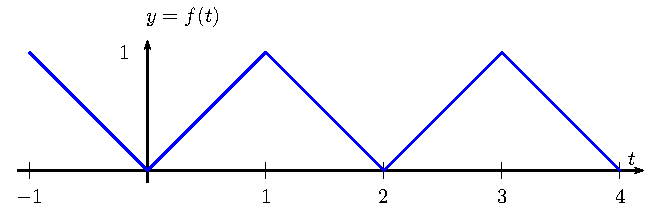
\includegraphics{figs/cap_series_figura_1}\end{center}
 Observamos que essa é uma função par, ou seja, $f(t)=f(-t)$. A fim de explorar essa simetria, utilizaremos as fórmulas (\ref{coef}) envolvendo integrais simétricas, isto é,
   \begin{eqnarray*}
    a_0&=& \frac{2}{T}\int_{-T/2}^{T/2} f(t)dt\\
    a_n&=&  \frac{2}{T}\int_{-T/2}^{T/2} f(t)\cos(w_nt)dt\\
    b_n&=&\frac{2}{T}\int_{-T/2}^{T/2} f(t)\sen(w_nt)dt
   \end{eqnarray*}
 onde $T=2$ e $w_n=\frac{2\pi n}{T}=\pi n$. Logo,
   \begin{equation*}
    a_0= \int_{-1}^{1} |t| dt=2\int_{0}^{1} t dt=2\left[\frac{t^2}{2}\right]_0^1=1\\
 	\end{equation*}
 	\begin{eqnarray*}
    a_n=  \int_{-1}^{1} |t|\cos(\pi n t)dt&=&2 \int_{0}^{1} t\cos(\pi n t)dt\\&=&2\left[\frac{t\sen(\pi n t)}{\pi n}\right]_0^1-2\int_0^1\frac{\sen(\pi n t)}{\pi n}dt\\
 	&=&2\left[\frac{t\sen(\pi n t)}{\pi n}+\frac{\cos(\pi n t)}{\pi^2 n^2}\right]_0^1=2\frac{(-1)^n-1}{\pi^2n^2}\\
 	 \end{eqnarray*}
 	\begin{eqnarray*}
    b_n&=&\int_{-1}^{1} |t|\sen(\pi n t)dt=0.
   \end{eqnarray*}
 onde se usou que $|t|$, $|t|\cos(\pi n t)$ são funções pares em $t$ e $|t|\sen(\pi n t)$ é ímpar em $t$. Assim, temos
 \begin{equation}
 f(t)=\frac{1}{2}-\frac{4}{\pi^2}\left(\cos(\pi t)+\frac{1}{3^2}\cos(3\pi t)+\frac{1}{5^2}\cos(5\pi t)+\cdots\right)
 \end{equation}
 Observe que, quando $t=0$, obtemos como subproduto da série de Fourier da $f(t)$ a soma da seguinte série numérica:
 \begin{equation}\label{serie_inv_impar}
 1+\frac{1}{3^2}+\frac{1}{5^2}+\cdots=\frac{\pi^2}{8}.
 \end{equation}
 A figura \ref{fig_conv_triangular} apresenta os gráficos da série que representa a função $f(t)$ com um termo, dois termos e três termos.
 \begin{figure}[!ht]
 \begin{center}
 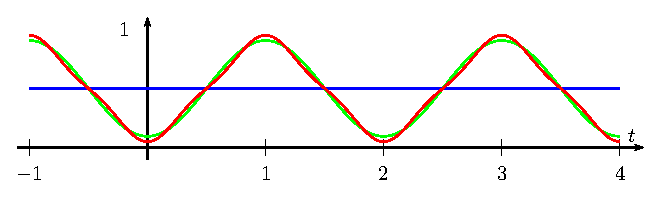
\includegraphics{figs/cap_series_figura_2}\end{center}
 \caption{\label{fig_conv_triangular}Gráficos de $f_0(t)=\frac{1}{2}$ (azul), $f_1(t)=\frac{1}{2}-\frac{4}{\pi^2}\cos(\pi t)$ (verde) e $f_2(t)=\frac{1}{2}-\frac{4}{\pi^2}\left(\cos(\pi t)+\frac{1}{3^2}\cos(3\pi t)\right)$ (vermelho).}
 \end{figure}

 {\bf Onda quadrada}

 Seja $g(t)$ uma função dada por
 \begin{eqnarray*}
 g(t)&=&-1, \ \ -1< t<0\\
 g(t)&=&0, \ \ t=0\ \hbox{ou}\ t=1\\
 g(t)&=&1, \ \ 0< t<1\\
 g(t+2)&=&g(t),\ \ \forall t\in\mathbb{R}.
 \end{eqnarray*}
 Essa função é suave por partes e contínua em todos os pontos exceto por saltos nos inteiros, onde a função vale a média aritmética dos limites laterais. Portanto se aplica o teorema \ref{teo_Dirichlet}.
 \begin{figure}[!ht]
 \begin{center}
 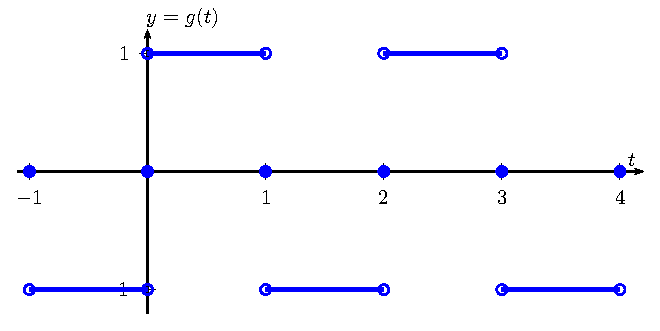
\includegraphics{figs/cap_series_figura_3}\end{center}
 \end{figure}
 Observamos que essa é uma função ímpar, ou seja, $f(t)=-f(-t)$. Novamente, utilizaremos as fórmulas (\ref{coef}) envolvendo integrais simétricas:
   \begin{equation*}
    a_0= \int_{-1}^{1} g(t) dt=0\\
 	\end{equation*}
 	\begin{eqnarray*}
    a_n=  \int_{-1}^{1} g(t)\cos(\pi n t)dt=0\\
 	 \end{eqnarray*}
 	\begin{eqnarray*}
    b_n=\int_{-1}^{1} g(t)\sen(\pi n t)dt=2\int_{0}^{1} g(t)\sen(\pi n t)dt&=&2\int_{0}^{1} \sen(\pi n t)dt\\
 	&=&\frac{2}{\pi n}\left[-\cos(\pi n t)\right]_0^1=2\frac{1-(-1)^n}{\pi n}
   \end{eqnarray*}

    Logo,
 \begin{equation}
 g(t)=\frac{4}{\pi}\left(\sen(\pi t)+\frac{1}{3}\sen(3\pi t)+\frac{1}{5}\sen(5\pi t)+\cdots\right).
 \end{equation}
 A figura \ref{fig_conv_quadrangular} apresenta os gráficos da série que representa a função $g(t)$ com um termo, dois termos, três termos e quatro termos.
 \begin{figure}[!ht]
 \begin{center}
 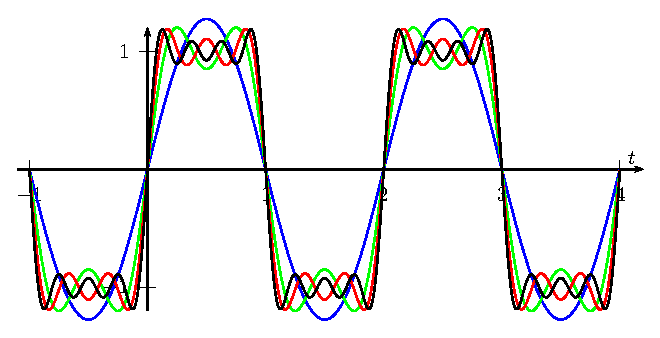
\includegraphics{figs/cap_series_figura_4}\end{center}
 \caption{\label{fig_conv_quadrangular}Gráficos de $g_0(t)=\frac{4}{\pi}\sen(\pi t)$ (azul), $g_1(t)=\frac{4}{\pi}\left(\sen(\pi t)+\frac{1}{3}\sen(3\pi t)\right)$ (verde), $g_2(t)=g(t)=\frac{4}{\pi}\left(\sen(\pi t)+\frac{1}{3}\sen(3\pi t)+\frac{1}{5}\sen(5\pi t)\right)$ (vermelho) e $g_3(t)=g(t)=\frac{4}{\pi}\left(\sen(\pi t)+\frac{1}{3}\sen(3\pi t)+\frac{1}{5}\sen(5\pi t)+\frac{1}{7}\sen(7\pi t)\right)$ (preto).}
\end{figure}

{\bf Exemplo} Seja $h(t)$ uma função dada por
 \begin{eqnarray*}
 f(t)&=&t, \ \ 0<t<1\\
 f(t)&=&\frac{1}{2}, \ \ t=1\\
 f(t+1)&=&f(t),\ \ \forall t\in\mathbb{R}.
 \end{eqnarray*}
 Essa função é suave por partes e contínua exceto por salto nos inteiros onde $h(t)$ assume o valor médio dos limites laterais. Portanto se aplica o teorema \ref{teo_Dirichlet}.
 \begin{figure}[!ht]
 \begin{center}
 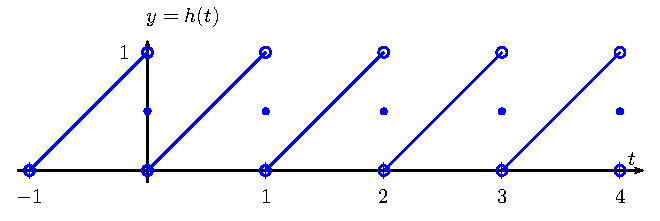
\includegraphics{figs/cap_series_figura_5}\end{center}
 \end{figure}
 Utilizaremos as fórmulas (\ref{coef}) envolvendo integrais no intervalo $[0,1]$, isto é,
   \begin{equation*}
    a_0= 2\int_{0}^{1} t dt=2\left[\frac{t^2}{2}\right]_0^1=1\\
 	\end{equation*}
 	\begin{eqnarray*}
    a_n=  2\int_{0}^{1} t\cos(2 \pi n t)dt=&=&2\left[\frac{t\sen(2 \pi n t)}{2 \pi n}\right]_0^1-2\int_0^1\frac{\sen(2 \pi n t)}{2 \pi n}dt\\
 	&=&2\left[\frac{t\sen(2 \pi n t)}{2 \pi n}+\frac{\cos(2 \pi n t)}{4\pi^2 n^2}\right]_0^1=0\\
 	 \end{eqnarray*}
 	\begin{eqnarray*}
    b_n=  2\int_{0}^{1} t\sen(2 \pi n t)dt=&=&2\left[-\frac{t\cos(2 \pi n t)}{2 \pi n}\right]_0^1+2\int_0^1\frac{\cos(2 \pi n t)}{2 \pi n}dt\\
 	&=&2\left[-\frac{t\cos(2 \pi n t)}{2 \pi n}+\frac{\sen(2 \pi n t)}{4\pi^2 n^2}\right]_0^1=-\frac{1}{\pi n}\\
 	 \end{eqnarray*}
 Logo,
 \begin{equation}
 h(t)=\frac{1}{2}-\frac{1}{\pi}\left(\sen(2 \pi t)+\frac{1}{2}\sen(4\pi t)+\frac{1}{3}\sen(6\pi t)+\cdots\right).
 \end{equation}

 
 {\bf Obs:} Os coeficiente $b_n$ da série de Fourier de uma função par são nulos bem como os coeficiente $a_n$ da série de Fourier de uma função ímpar também o são.

Demonstre a observação .




 \chapter{21 de outubro}
\subsection{Diagramas de espectro}


Diagramas espectro são representações gráficas dos coeficientes de Fourier $C_n$ associados a uma função periódica $f(t)$. Como os coeficientes $C_n$ são números complexos, é comum representá-los na forma de módulo e fase, isto é:
 \begin{equation}C_n = |C_n|e^{i\phi_n}.\end{equation}
 O ângulo de fase assim definido coincide com o conceito de argumento do número $C_n$.

 {\bf Exemplo:} A função 
 \begin{equation}f(t)=-1+2\cos(t)+4\sen(2t)\end{equation}
 é periódica com periodo fundamental $2\pi$ e pode ser escrita na forma exponencial da seguinte forma:
 \begin{eqnarray*}
 f(t)&=&-1+2\left(\frac{e^{it}+e^{-it}}{2}\right)+4\left(\frac{e^{2it}-e^{-2it}}{2i}\right)\\
 &=&2i e^{-2it} + e^{-it}-1+e^{it}- 2ie^{2it}
 \end{eqnarray*}
 Assim, identificamos cinco coeficientes não nulos:
 \begin{equation*}
 \begin{array}{lclcll}
  C_{-2}&=&2i=2e^{\frac{i\pi}{2}} &\Longrightarrow& |C_{-2}|=2, ~~ &\phi_{-2}=\frac{\pi}{2}\\
  C_{-1}&=&1 &\Longrightarrow& |C_{-1}|=1, ~~ &\phi_{-1}=0\\
  C_{0}&=&-1=1e^{\pi} &\Longrightarrow& |C_{0}|=1, ~~ &\phi_0=\pi\\
  C_{1}&=&1 &\Longrightarrow& |C_{1}|=1, ~~ &\phi_1=0\\
  C_{2}&=&-2i=2e^{\frac{-i\pi}{2}} &\Longrightarrow& |C_{2}|=2, ~~ &\phi_2=-\frac{\pi}{2}
 \end{array}
  \end{equation*}
 Os digramas de espectro de amplitude e fase são dados a seguir:
 \begin{figure}[!ht]
 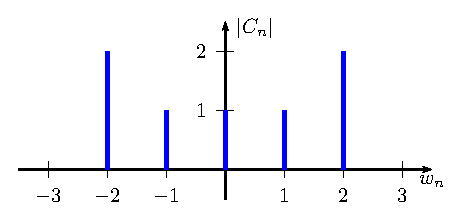
\includegraphics{figs/cap_diagramas_espectro_figura_2}
 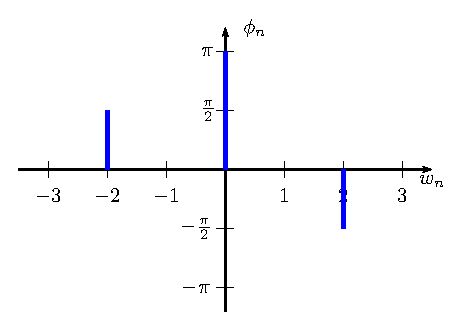
\includegraphics{figs/cap_diagramas_espectro_figura_3}
 \end{figure}

 
{\bf Exemplo:} As primeiras raias do diagrama de espectro da função a seguir: 
 \begin{equation}
 g(t)=\cdots+\frac{2i}{5\pi}e^{-5i\pi t}+\frac{2i}{3\pi}e^{-3i\pi t}+\frac{2i}{\pi}e^{-i\pi t}-\frac{2i}{\pi}e^{i\pi t}-\frac{2i}{3\pi}e^{3i\pi t}-\frac{2i}{5\pi}e^{5i\pi t}-\cdots,
 \end{equation}
 são dados na figura a seguir
 \begin{figure}[!ht] 
 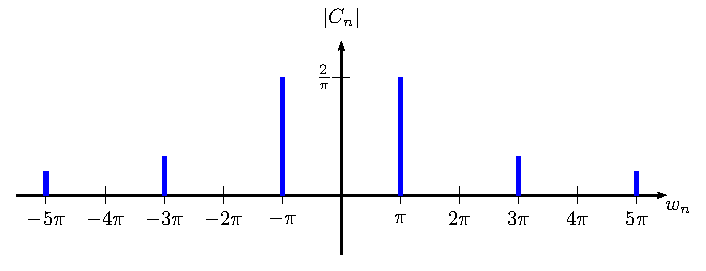
\includegraphics{figs/cap_diagramas_espectro_figura_4}
 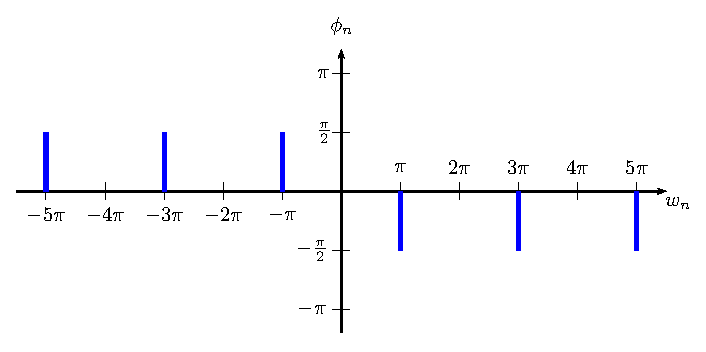
\includegraphics{figs/cap_diagramas_espectro_figura_5}
 \end{figure}


 {\bf Exemplos:}
 
 $$f(t)=\sum_{n=1}^\infty \frac{1}{n^2}\cos(nt)$$
 
 $$g(t)=\sum_{n=1}^\infty \frac{1}{n^2}\sin(nt)$$
 
 
 \section{Propriedades das Séries de Fourier}
 
Define-se a potência média de um função periódica $f(t)$ como
\begin{equation}\overline{P}_f=\frac{1}{T}\int_0^T |f(t)|^2dt
\end{equation}

 A potência média da função $f(t)=A\cos(wt)$ é dada por
 \begin{eqnarray*}
 \overline{P}_f&=&\frac{1}{T}\int_0^T |f(t)|^2dt\\
 &=&\frac{1}{T}\int_0^{T} A^2\cos\left(\frac{2\pi}{T} t\right)^2dt\\
 &=&\frac{A^2}{T}\int_0^{T} \left(\frac{\cos\left(\frac{4\pi}{T} t\right)+1}{2}  \right)dt\\
 &=&\frac{A^2}{2}
 \end{eqnarray*}
  onde se usou que $w=\frac{2\pi}{T}$ e identidade trigonométrica dada por:
 \begin{equation}\cos^2(x)=\left(\frac{e^{ix}+e^{-ix}}{2}\right)^2=\frac{e^{2ix}+2+e^{-2ix}}{4}=\frac{\cos(2x)+1}{2}.\end{equation}

{\bf Exemplo:} Seja $V(t)=A\cos(wt)$ uma fonte de tensão com frequência $w=60$\ \!\!Hz $=120\pi$\ \!\!rad/s ligado a um resistor de resistência $R\Omega$. A potência no resistor é
 \begin{equation}
 P(t)=\frac{V(t)^2}{R}
 \end{equation}
 e a potência média $P_m$ é
 \begin{equation}
 P_m=\frac{1}{T}\int_0^TP(t)dt=\frac{1}{T}\int_0^T\frac{V(t)^2}{R}dt,
 \end{equation}
 onde $T=\frac{1}{60}s$. Por outro lado, a potência média é calculada em termos da tensão média por
 \begin{equation}
 P_m=\frac{V_m^2}{R},
 \end{equation}
 ou seja,
 \begin{equation}{\label{valor_RMS}}
 V_m^2=\frac{1}{T}\int_0^T V(t)^2 dt.
 \end{equation}
 O exemplo  nos dá o valor da potência média do sinal $V(t)=A\cos(wt)$. Logo,
 \begin{equation}
 V_m=\frac{A}{\sqrt{2}}.
 \end{equation}
 Se $V_m=127V$, então a amplitude do sinal é aproximadamente $A\approx 180$.

 
{\bf Observação:}
Na expressão (\ref{valor_RMS}), $V_m$ também é chamado de valor RMS do sinal $v(t)$ (Root mean square):
 \begin{equation}
 V_{RMS}=\sqrt{\frac{1}{T}\int_0^T V(t)^2 dt}.
 \end{equation}

 {\bf Teorema de Parseval} Seja $f(t)$ uma função periódica representável por uma série de Fourier, então vale a seguinte identidade.
 \begin{equation}\label{teo_parseval} 
 \frac{1}{T}\int_0^T |f(t)|^2dt=\sum_{n=-\infty}^\infty |C_n|^2.
  \end{equation}

{\bf Dem:}
 \begin{eqnarray*}
  \frac{1}{T}\int_0^T |f(t)|^2dt&=&\frac{1}{T}\int_0^T f(t)\overline{f(t)}dt
 \end{eqnarray*}
  Como $\displaystyle f(t)=\sum_{n=-\infty}^\infty C_n e^{iw_n t}$, temos
  \begin{eqnarray*}
   \overline{f(t)}&=&\overline{\sum_{n=-\infty}^\infty C_n e^{iw_n t}}
   =\sum_{n=-\infty}^\infty \overline{C_n}~ \overline{e^{iw_n t}}
   =\sum_{n=-\infty}^\infty \overline{C_n} e^{-iw_n t}
  \end{eqnarray*}
 Substituindo esta expressão para $\overline{f(t)}$ na definição de potência média, temos:
 \begin{eqnarray*}
  \frac{1}{T}\int_0^T |f(t)|^2dt&=&\frac{1}{T}\int_0^T f(t)\overline{f(t)}dt=\frac{1}{T}\int_0^Tf(t)\left[\sum_{n=-\infty}^\infty \overline{C_n} e^{-iw_n t}\right] dt\\
  &=&\frac{1}{T}\sum_{n=-\infty}^\infty\left[\overline{C_n}\int_0^Tf(t)e^{-iw_nt}dt\right]
  \end{eqnarray*}
  Como $C_n=\frac{1}{T}\int_0^Tf(t)e^{-iw_nt}dt$, temos:
 \begin{eqnarray*}
  \frac{1}{T}\int_0^T |f(t)|^2dt&=&\sum_{n=-\infty}^\infty\overline{C_n}C_n = \sum_{n=-\infty}^\infty|C_n|^2
  \end{eqnarray*}







 
 {\bf Exemplo}
Seja $g(t)$ um função dada no exemplo \ref{ex_quadrada}, isto é,
 \begin{eqnarray*}
 g(t)&=&-1, \ \ -1< t<0\\
 g(t)&=&0, \ \ t=0\ \hbox{ou}\ t=1\\
 g(t)&=&1, \ \ 0< t<1\\
 g(t+2)&=&g(t),\ \ \forall t\in\mathbb{R}.
 \end{eqnarray*}
 \begin{figure}[!ht]
 \begin{center}
 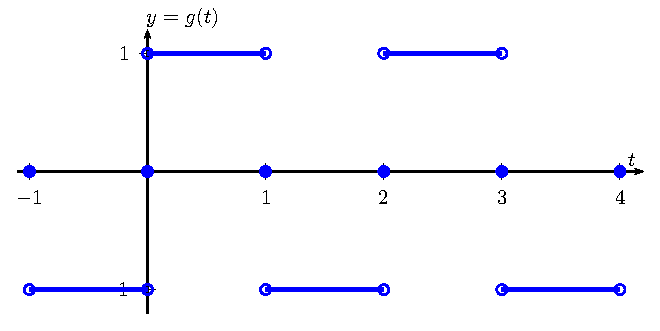
\includegraphics{figs/cap_propriedades_series_figura_1}\end{center}
 \end{figure}
 Vimos no exemplo \ref{ex_quadrada} que sua expansão em série de Fourier é da forma:
 \begin{equation}
 g(t)=\frac{4}{\pi}\left(\sen(\pi t)+\frac{1}{3}\sen(3\pi t)+\frac{1}{5}\sen(5\pi t)+\cdots\right).
 \end{equation}
 Calcularemos agora a potência média desta função através de sua representação no tempo e depois em frequência:
 \begin{eqnarray*}
  \overline{P_f}=\frac{1}{T}\int_0^T |g(t)|^2dt=\frac{1}{2}\int_0^2 |g(t)|^2dt=\frac{1}{2}\int_0^2 1dt=1
 \end{eqnarray*}
 Alternativamente, temos pelo Teorema de Parseval:
 \begin{eqnarray*}
  \overline{P_f}=\sum_{n=-\infty}^\infty |C_n|^2=\sum_{n=-\infty}^\infty \left|\frac{a_n-ib_n}{2}\right|^2=\frac{1}{4}\sum_{n=-\infty}^\infty |b_n|^2
 \end{eqnarray*}
 Como $b_{-n}=b_n$, temos que $|b_{-n}|=|b_n|$ e ainda temos que $b_0=0$, portanto: 
 \begin{eqnarray*}
  \overline{P_f}=\frac{1}{2}\sum_{n=1}^\infty |b_n|^2 = \frac{1}{2}\left(\frac{4}{\pi}\right)^2\left(1 + \frac{1}{3^2}+ \frac{1}{5^2}+ \frac{1}{7^2}+\cdots\right)
 \end{eqnarray*}
 temos:
 \begin{eqnarray*}
  \overline{P_f}=\frac{1}{2}\left(\frac{4}{\pi}\right)^2\frac{\pi^2}{8}=1
 \end{eqnarray*}

 
 
 
 
 
 
 
 
 
 
 
 
 \section{Passagem do discreto para o contínuo}
 
 \chapter{23 de outubro}
 \section{Exemplos de transformadas de Fourier}
 
 
 
\subsection{Função tenda assimétrica}

 \begin{equation}f(t)=\left\{\begin{array}{cc}e^{at}&\hbox{se}\ t<0\\
 e^{-bt}&\hbox{se}\ t>0
 \end{array}\right.
 \end{equation}
 onde $a$ e $b$ são constantes positivas. A figura  mostra o gráfico de $f(t)$ para $a=1$ e $b=3$.
 \begin{figure}[!ht]
 \begin{center}
 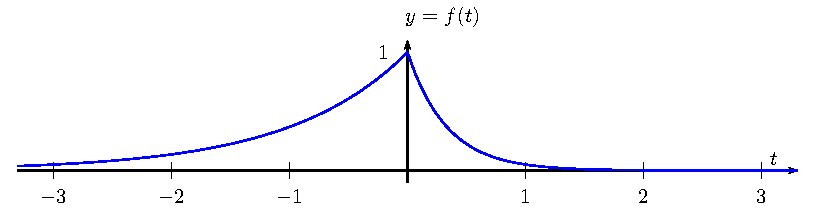
\includegraphics{figs/cap_transformada_de_fourier_figura_7}\end{center}
 \caption{\label{fig_trans_1} Gráfico de $f(t)=e^{t}$, se $t<0$ ou $f(t)=e^{-3t}$ se $t>0$.  }
 \end{figure}
 A transformada de Fourier de $f(t)$ é calculada da seguinte forma:
 \begin{eqnarray*}
 F(w)=\mathcal{F}\{f(t)\}&=&\int_{-\infty}^\infty f(t) e^{-i w t}dt\\
 &=&\int_{-\infty}^0 e^{at} e^{-i w t}dt+\int_{0}^\infty e^{-bt} e^{-i w t}dt\\
 &=&\int_{-\infty}^0 e^{at} \left(\cos(wt)-i\sen(wt)\right)dt+\int_{0}^\infty e^{-bt} \left(\cos(wt)-i\sen(wt)\right)dt\\
 &=&\int_{0}^\infty e^{-at} \left(\cos(wt)+i\sen(wt)\right)dt+\int_{0}^\infty e^{-bt} \left(\cos(wt)-i\sen(wt)\right)dt\\
 &=&\frac{a}{a^2+w^2}+\frac{iw}{a^2+w^2}+\frac{b}{b^2+w^2}-\frac{iw}{b^2+w^2}\\
 &=&\frac{a}{a^2+w^2}+\frac{b}{b^2+w^2}+i\left(\frac{w}{a^2+w^2}-\frac{w}{b^2+w^2}\right)
 \end{eqnarray*}
 onde se usou os itens 1 e 2 da tabela de integrais definidas.

 {\bf O que acontece quando $a=b$?}
 % 
% 
 \subsection{Delta de Dirac}
 
 Calculamos a transformada de Fourier do delta de Dirac $\delta(t-a)$, $a\in\mathbb{R}$ da seguinte forma:
 \begin{eqnarray*}
 F(w)=\mathcal{F}\{\delta(t-a)\}&=&\int_{-\infty}^\infty \delta(t-a) e^{-i w t}dt\\
 &=&e^{-i w a}
 \end{eqnarray*}

 \chapter{23 de outubro}
  \section{Forma trigonométrica}
 A forma exponencial da transformada de Fourier de uma função $f(t)$ foi definida no capítulo \ref{trans_Fourier} e é dada por
 \begin{equation}
 F(w)=\mathcal{F}\{f(t)\}=\int_{-\infty}^\infty f(t)e^{-iwt}dt.
 \end{equation}
 Se $f(t)$ é uma função real, então podemos separar a parte real e imaginária da transformada de Fourier, conforme a seguir:
 \begin{eqnarray*}
 F(w)&=&\mathcal{F}\{f(t)\}=\int_{-\infty}^\infty f(t)e^{-iwt}dt\\
 &=&\int_{-\infty}^\infty f(t)\left(\cos(wt)-i\sen(wt)\right)dt\\
 &=&\int_{-\infty}^\infty f(t)\cos(wt)dt-i\int_{-\infty}^\infty f(t)\sen(wt) dt\\
 &:=&A(w)-iB(w),
 \end{eqnarray*}
 onde
 \begin{eqnarray*}
 A(w)&=&\int_{-\infty}^\infty f(t)\cos(wt)dt\\
 B(w)&=&\int_{-\infty}^\infty f(t)\sen(wt) dt
 \end{eqnarray*}
 Nesses termos, a função $f(t)$ pode ser escrita como:
 \begin{eqnarray*}
 f(t)&=&\frac{1}{2\pi}\int_{-\infty}^\infty F(w)e^{iwt}dw\\
 &=&\frac{1}{2\pi}\int_{-\infty}^\infty \left(A(w)-i B(w)\right)\left(\cos(wt)+i\sen(wt)\right)dw\\
 &=&\frac{1}{2\pi}\int_{-\infty}^\infty\left( A(w)\cos(wt)+ B(w)\sen(wt)\right)dw\\&+&\frac{i}{2\pi}\int_{-\infty}^\infty \left(A(w)\sen(wt)- B(w)\cos(wt)\right)dw
 \end{eqnarray*}
 Usando o fato que $A(w)$ é uma função par e $B(w)$ é uma função ímpar, temos:
 \begin{eqnarray*}
 f(t)&=&\frac{1}{2\pi}\int_{-\infty}^\infty\left(A(w)\cos(wt)+ B(w)\sen(wt)\right)dw\\
 &=&\frac{1}{\pi}\int_{0}^\infty\left( A(w)\cos(wt)+ B(w)\sen(wt)\right)dw
 \end{eqnarray*}
 A tabela abaixo compara as formas trigonométrica e exponencial das séries e transformadas de Fourier
 \begin{equation}
 \begin{array}{|c|c|c|}
 \hline &&\\
 &\hbox{Forma exponencial}&\hbox{Forma trigonométrica}\\&&\\  \hline &&\\
 \hbox{Série de Fourier}&\displaystyle f(t)=\sum_{n=-\infty}^\infty C_n e^{i w_n t} & \displaystyle  f(t)=\frac{a_0}{2}+\sum_{n=1}^\infty\left( a_n \cos(w_nt)+b_n\sen(w_nt)\right)   \\&&\\\hline &&\\
 \hbox{Transformada de Fourier} &\displaystyle f(t)=\frac{1}{2\pi}\int_{-\infty}^\infty F(w)e^{iwt}dw &\displaystyle f(t)=\frac{1}{\pi}\int_{0}^\infty \left( A(w)\cos(wt)+ B(w)\sen(wt)\right)dw \\   &&\\\hline
 \end{array}
 \end{equation}

 {\bf Exemplo:} Considere a função $f(t)=e^{-at}u(t)$ onde $a$ é uma constante positiva e $u(t)$ é a função Heaviside. A transformada de Fourier $F(w)$ de $f(t)$ foi calculada como exercício e é dada por:
 \begin{equation*}
 F(w)=\frac{a}{a^2+w^2}-\frac{iw}{a^2+w^2}.
 \end{equation*}
 Usando representação trigonométrica da transformada de Fourier, temos:
 \begin{eqnarray*}
 f(t)=\frac{1}{\pi}\int_{0}^\infty\left( A(w)\cos(wt)+ B(w)\sen(wt)\right)dw,
 \end{eqnarray*}
 onde
 \begin{eqnarray*}
 A(w)&=&\frac{a}{a^2+w^2}\\
 B(w)&=&\frac{w}{a^2+w^2}
 \end{eqnarray*}

 
 \section{Diagramas de espectro}
Diagrama de espectro da transformada de Fourier é a representação gráfica da transformada de Fourier $F(w)$ associadas a uma função $f(t)$. Da mesma forma como o diagrama de espectro da série de Fourier se divide em amplitude e fase, o diagrama de espectro da transformada de Fourier se divide em magnitude e fase. Ou seja, o gráfico de $|F(w)|$ é a diagrama de magnitude e o gráfico de $\phi(w)$ é o diagrama de fase, onde
\begin{equation}
F(w)=|F(w)|e^{i\phi(w)},
\end{equation}
Já calculamos a transformada de Fourier da função $f(t)=e^{-|t|}$:
 \begin{equation}
 F(w)=\frac{2}{w^2+1}.
 \end{equation}
 O gráfico da magnitude $|F(w)|$ é dado na figura. Devido o fato de $F(w)$ ser real, a fase é uma função nula.
 \begin{figure}[!ht]
 \begin{center}
 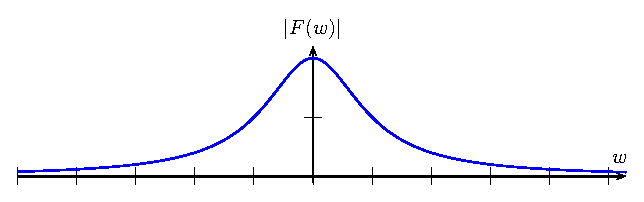
\includegraphics{figs/cap_diagramas_espectro_transformada_figura_1}\end{center}
 \end{figure}

A transformada de Fourier da função $f(t)=e^{-at}u(t)$ onde $a$ é uma constante positiva e $u(t)$ é a função Heaviside é dado por: 
 \begin{equation*}
 F(w)=\frac{a}{a^2+w^2}-\frac{iw}{a^2+w^2}.
 \end{equation*}
 Observe que
 \begin{eqnarray*}
 |F(w)|&=&\sqrt{\left(\frac{a}{a^2+w^2}\right)^2+\left(\frac{w}{a^2+w^2}\right)^2}\\
 &=&\sqrt{\frac{a^2+w^2}{\left(a^2+w^2\right)^2}}\\&=&\frac{1}{\sqrt{a^2+w^2}}
 \end{eqnarray*}
 e, como $a>0$, temos $\frac{a}{a^2+w^2}>0$. Portanto,
 \begin{equation}
 \phi(w)=\tan^{-1}\left(\frac{-\frac{w}{a^2+w^2}}{\frac{a}{a^2+w^2}}\right)=-\tan^{-1}\left(\frac{w}{a}\right).
 \end{equation}
 A figura \ref{diag_espec_trans_2} apresenta o diagrama de espectro de magnitude e fase da transformada $F(w)$ de $f(t)$ quando $a=1$.
  \begin{figure}[!ht]
  \begin{center}
  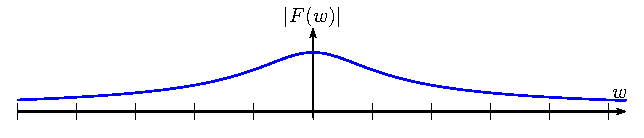
\includegraphics{figs/cap_diagramas_espectro_transformada_figura_2}
  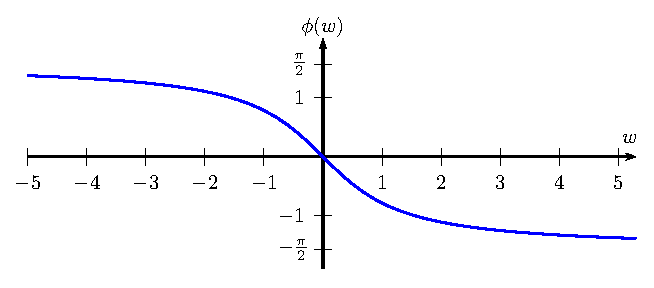
\includegraphics{figs/cap_diagramas_espectro_transformada_figura_3}\end{center}
  \caption{\label{diag_espec_trans_2}}
  \end{figure}

  
  \chapter{23 de outubro - Propriedades I - }
    
  \section{Linearidade}
  
Dadas duas funções $f(t)$ e $g(t)$ com transformadas de Fourier $F(w)$ e $G(w)$, respectivamente, e $\alpha$ e $\beta$ duas constantes reais ou complexas, então
\begin{equation}
\mathcal{F}\left\{\alpha f(t)+\beta g(t)\right\}=\alpha \mathcal{F}\{ f(t)\}+\beta\mathcal{F}\{ g(t)\}=\alpha F(w)+\beta G(w)
\end{equation}
  
  \section{Derivada}
   Dada uma função diferenciável $f(t)$ tal que 
\begin{equation}\lim_{t\to \pm \infty}f(t)=0
\end{equation}
e sua transformada de Fourier $F(w)$, então
\begin{equation}
\mathcal{F}\{f'(t)\}=iw F(w)
\end{equation}

\subsection{Exemplo}
 Considere a função $f(t)=e^{-at^2}$, $a>0$, e sua transformada de Fourier:
\begin{equation}
F(w)=\frac{\sqrt{\pi}}{\sqrt{a}}e^{-\frac{w^2}{4a}}
\end{equation}
Usando a propriedade da derivada, a transformada de Fourier da derivada $f'(t)=-2 a t e^{-at^2}$ é dada por:
\begin{equation}
\mathcal{F}\{-2 a t e^{-at^2} \}=iwF(w)=iw\frac{\sqrt{\pi}}{\sqrt{a}}e^{-\frac{w^2}{4a}}.
\end{equation}
Usando a linearidade, encontramos a transformada de Fourier da função $t e^{-at^2}$:
\begin{equation}
\mathcal{F}\{  t e^{-at^2} \}=-iw\frac{\sqrt{\pi}}{2a\sqrt{a}}e^{-\frac{w^2}{4a}}.
\end{equation}

% 
% 
\section{Deslocamento no eixo $w$} Dada uma função $f(t)$ e sua transformada de Fourier $F(w)$, então
 \begin{equation}
 \mathcal{F}\left\{e^{at}f(t)\right\}=F(w+ia).
 \end{equation}

 De fato,
 \begin{eqnarray*}
 \mathcal{F}\left\{e^{at}f(t)\right\}&=&\int_{-\infty}^\infty  f(t)e^{at}e^{-iwt}dt \\
 &=&\int_{-\infty}^\infty   f(t)e^{(a-iw)t}dt \\
 &=&\int_{-\infty}^\infty   f(t)e^{-i(ia+w)t}dt \\
 &=&F(w+ia) 
 \end{eqnarray*}

A transformada de Fourier da função $f(t)=t e^{-at^2}$, $a>0$, é dada por
 \begin{equation}
 F(w)=-iw\frac{\sqrt{\pi}}{2a\sqrt{a}}e^{-\frac{w^2}{4a}}.
 \end{equation}
 Logo, a transformada $G(w)$ da função $g(t)=t e^{bt-at^2}$, $b>0$, é dada por
 \begin{eqnarray*}
 G(w)=\mathcal{F}\left\{t e^{bt-at^2}\right\}&=&\mathcal{F}\left\{e^{bt}t e^{-at^2}\right\}\\
 &=&F(w+ib)\\
 &=&-i(w+ib)\frac{\sqrt{\pi}}{2a\sqrt{a}}e^{-\frac{(w+ib)^2}{4a}}\\
 &=&(b-iw)\frac{\sqrt{\pi}}{2a\sqrt{a}}e^{-\frac{w^2+2wib-b^2}{4a}}\\
 &=&\sqrt{w^2+b^2}e^{-i\arctan\left(\frac{w}{b}\right)}\frac{\sqrt{\pi}}{2a\sqrt{a}}e^{-\frac{w^2-b^2}{4a}}e^{-i\left(\frac{wb}{2a}\right)}\\
 &=&\sqrt{w^2+b^2}\frac{\sqrt{\pi}}{2a\sqrt{a}}e^{-\frac{w^2-b^2}{4a}}e^{-i\left(\frac{wb}{2a}+\arctan\left(\frac{w}{b}\right)\right)}\\
 &=&|G(w)|e^{i\phi(w)},
 \end{eqnarray*}
 onde
 \begin{eqnarray*}
 |G(w)|=\frac{\sqrt{\pi}}{2a\sqrt{a}}e^{-\frac{b^2}{4a}}\sqrt{w^2+b^2}e^{-\frac{w^2}{4a}}\qquad\hbox{ e }\qquad \phi(w)=-\left(\frac{wb}{2a}+\arctan\left(\frac{w}{b}\right)\right)
 \end{eqnarray*}
 Veja os diagramas de espectro de $G(w)$ quando $a=b=1$ na figura.
 \begin{figure}[!ht]
 \begin{center}
 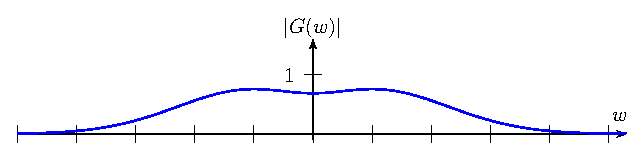
\includegraphics{figs/cap_propriedades_transformada_figura_2}
 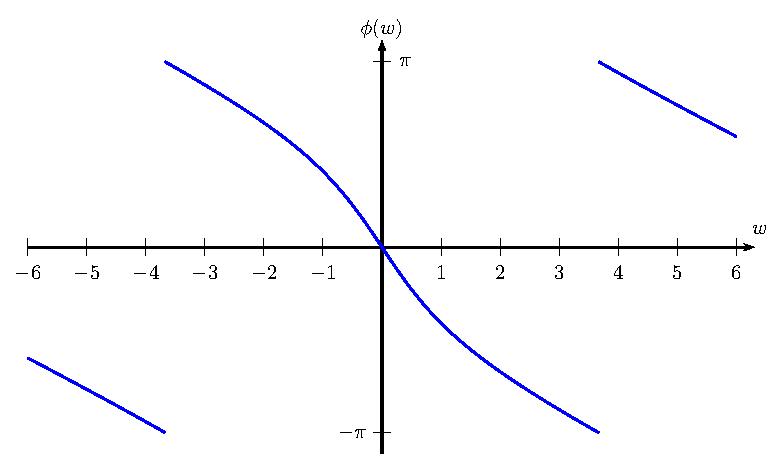
\includegraphics{figs/cap_propriedades_transformada_figura_3}\end{center}
 \caption{\label{diag_espec_trans_4}}
 \end{figure}

\section{Deslocamento no eixo $t$}

Dada uma função $f(t)$ e sua transformada de Fourier $F(w)$, então
 \begin{equation}
 \mathcal{F}\left\{f(t-a)\right\}=e^{-iaw}F(w).
 \end{equation}
 
 De fato,
 \begin{eqnarray*}
 \mathcal{F}\left\{f(t-a)\right\}&=&\int_{-\infty}^\infty  f(t-a)e^{-iwt}dt \\
 &=&\int_{-\infty}^\infty  f(s)e^{-iw(s+a)}ds \\
 &=&\int_{-\infty}^\infty  f(s)e^{-iwa}e^{-iws}ds \\
 &=&e^{-iwa}\int_{-\infty}^\infty  f(s)e^{-iws}ds \\
 &=&e^{-iaw}F(w)
 \end{eqnarray*}

 
A transformada de Fourier da função $f(t)=e^{-|t|}$ é dada por $F(w)=\frac{2}{w^2+1}$. Logo, a transformada de Fourier da função $g(t)=e^{-|t-2|}$ é
 \begin{equation}
 G(w)=\frac{2}{w^2+1}e^{-2iw}
 \end{equation}

  {\bf Obs:} Um deslocamento real no tempo não altera o módulo da transformada de Fourier, pois $|e^{-iaw}|=1$ sempre que $a$ e $w$ são reais.

\section{Transformada da integral}
  Dada uma função integrável $f(t)$ tal que sua transformada de Fourier $F(w)$ satisfaça $F(0)=0$, então
   \begin{equation}
 \mathcal{F}\left\{\int_{-\infty}^t f(\tau)d\tau \right\}=\frac{1}{iw}F(w).
 \end{equation}

{\bf Dem:}
 Definimos $g(t)=\int_{-\infty}^t f(\tau)d\tau$ e, usando o teorema fundamental do cálculo, temos $g'(t)=f(t)$. Aplicamos a transformada de Fourier na igualdade e temos:
 \begin{equation}
 \mathcal{F}\{g'(t)\}=\mathcal{F}\{f(t)\},
 \end{equation}
 ou seja,
 \begin{equation}
 \mathcal{F}\{g'(t)\}=F(w).
 \end{equation}
 Observe que
 \begin{equation}
 \lim_{t\to\infty} g(t)=\int_{-\infty}^\infty f(\tau)d\tau=\int_{-\infty}^\infty f(\tau)e^{i\cdot 0 \cdot \tau}d\tau=F(0)=0
 \end{equation}
 e
 \begin{equation}
 \lim_{t\to-\infty} g(t)=\int_{-\infty}^{-\infty} f(\tau)d\tau=0,
 \end{equation}
 portanto, podemos usar a propriedade \ref{prop_der} da transformada de Fourier da derivada e obter:
 \begin{equation}
 \mathcal{F}\{g'(t)\}=iw \mathcal{F}\{g(t)\}.
 \end{equation}
 Assim,
 \begin{equation}
 F(w)=iw \mathcal{F}\left\{\int_{-\infty}^t f(\tau)d\tau\right\}.
 \end{equation}
 Portanto,
 \begin{equation}
 \mathcal{F}\left\{\int_{-\infty}^t f(\tau)d\tau\right\}=\frac{1}{iw}F(w).
 \end{equation}

\section{Teorema da modulação}\label{prop_mod}
Dada uma função $f(t)$ e sua transformada de Fourier $F(w)$, então
 \begin{equation}
 \mathcal{F}\left\{f(t)\cos(w_0t) \right\}=\frac{1}{2}F(w-w_0)+\frac{1}{2}F(w+w_0),
 \end{equation}
 para $w_0\in\mathbb{R}$.

{\bf Dem}
 De fato,
 \begin{eqnarray*}
 \mathcal{F}\left\{f(t)\cos(w_0t) \right\}&=&\mathcal{F}\left\{f(t)\left(\frac{e^{iw_0t}+e^{-iw_0t}}{2} \right)\right\} \\
 &=&\int_{-\infty}^\infty f(t)\frac{e^{iw_0t}+e^{-iw_0t}}{2}e^{-iwt}dt  \\
 &=&\frac{1}{2}\int_{-\infty}^\infty f(t)e^{-i(w-w_0)t}dt+\frac{1}{2}  \int_{-\infty}^\infty f(t)e^{-i(w_0+w)t}dt\\
 &=&\frac{1}{2}F(w-w_0)+\frac{1}{2}F(w+w_0)
 \end{eqnarray*}

{\bf Exemplo:} Considere a função $f(t)=\cos(w_0t) e^{-a|t|}$, $a>0$. Podemos obter a transformada de Fourier de $f(t)$ a partir da transformada de Fourier da função $g(t)=e^{-a|t|}$. Basta aplicar o teorema da modulação à função $g(t)$, cuja transformada de Fourier é dada por $G(w)=\frac{2a}{w^2+a^2}$:
 \begin{eqnarray*}
 \mathcal{F}\left\{g(t)\cos(w_0t) \right\}&=&\frac{1}{2}G(w-w_0)+\frac{1}{2}G(w+w_0)\\
 &=&\frac{1}{2}\frac{2a}{(w-w_0)^2+a^2}+\frac{1}{2}\frac{2a}{(w+w_0)^2+a^2}\\
 &=&\frac{a}{(w-w_0)^2+a^2}+\frac{a}{(w+w_0)^2+a^2}
 \end{eqnarray*}

 \chapter{26 de outubro - Propriedades (continuação)}
\section{Teorema da convolução}
Dadas duas funções $f_1(t)$ e $f_2(t)$ com suas respectivas transformadas de Fourier, $F_1(w)$ e $F_2(w)$, então
 \begin{itemize}
 \item[a)] (Convolução no tempo)
 \begin{equation}\mathcal{F}\{(f_1*f_2)(t)\}=F_1(w)F_2(w),\end{equation}
 \item[b)] (Convolução na frequência)
 \begin{equation}(F_1*F_2)(w)=2\pi\mathcal{F}\{f_1(t)f_2(t)\}\end{equation}
 ou 
 \begin{equation}\mathcal{F}^{-1}\{(F_1*F_2)(w)\}=2\pi f_1(t)f_2(t),\end{equation}
 \end{itemize}
 onde $*$ indica a convolução de duas funções:
 \begin{equation}
 (f_1*f_2)(t)=\int_{-\infty}^\infty f_1(\tau)f_2(t-\tau)d\tau
 \end{equation}

 {\bf Observe} a definição de convolução.
 
{\bf Dem:}
 \begin{itemize}
 \item[a)] Usando as definições de transformada de Fourier e convolução de duas funções, temos:
 \begin{eqnarray}
 \nonumber \mathcal{F}\{(f_1*f_2)(t)\}&=&\int_{-\infty}^\infty (f_1*f_2)(t)e^{-iwt}dt\\
 \nonumber &=&\int_{-\infty}^\infty \left(\int_{-\infty}^\infty f_1(\tau)f_2(t-\tau)d\tau\right)e^{-iwt}dt\\
 &=&\int_{-\infty}^\infty \left[f_1(\tau) \int_{-\infty}^\infty f_2(t-\tau)e^{-iwt}dt\right]d\tau  {\label{eq_teo_conv}}
 \end{eqnarray}
 Uma das integrais pode ser calculada fazendo uma mudança de variável:
 \begin{eqnarray}
 \nonumber \int_{-\infty}^\infty f_2(t-\tau)e^{-iwt}dt&=&\int_{-\infty}^\infty f_2(s)e^{-iw(s+\tau)}ds \\
 \nonumber &=&e^{-iw\tau}\int_{-\infty}^\infty f_2(s)e^{-iws}ds \\
 &=&e^{-iw\tau}F_2(w) {\label{eq_teo_conv_1}}
 \end{eqnarray}
 Substituindo a equação (\ref{eq_teo_conv_1}) na equação (\ref{eq_teo_conv}), temos
 \begin{eqnarray*}
 \mathcal{F}\{(f_1*f_2)(t)\}&=&\int_{-\infty}^\infty \left[f_1(\tau) \int_{-\infty}^\infty f_2(t-\tau)e^{-iwt}dt\right]d\tau\\
 &=&\int_{-\infty}^\infty \left[f_1(\tau) e^{-iw\tau}F_2(w)\right]d\tau\\
 &=&F_2(w)\int_{-\infty}^\infty \left[f_1(\tau) e^{-iw\tau}\right]d\tau\\
 &=&F_1(w)F_2(w)
 \end{eqnarray*}
 \item[b)] Analogamente, usando as definições, temos:
 \begin{eqnarray}
 \nonumber\mathcal{F}^{-1}\{(F_1*F_2)(w)\}&=&\frac{1}{2\pi}\int_{-\infty}^\infty (F_1*F_2)(w)e^{iwt}dw\\
 \nonumber &=&\frac{1}{2\pi}\int_{-\infty}^\infty \left(\int_{-\infty}^\infty F_1(v)F_2(w-v)dv \right)e^{iwt}dw\\
 &=&\frac{1}{2\pi}\int_{-\infty}^\infty\left[ F_1(v) \int_{-\infty}^\infty F_2(w-v)e^{iwt}dw \right]dv {\label{eq_teo_conv_2}}
 \end{eqnarray}
 Também,
 \begin{eqnarray}
 \nonumber \int_{-\infty}^\infty F_2(w-v)e^{iwt}dw&=&\int_{-\infty}^\infty F_2(y)e^{i(y+v)t}dy \\
 \nonumber &=&e^{ivt}\int_{-\infty}^\infty F_2(y)e^{iyt}dy \\
 &=&2\pi e^{ivt}f_2(t) {\label{eq_teo_conv_3}}
 \end{eqnarray}
 Substituindo a equação (\ref{eq_teo_conv_3}) na equação (\ref{eq_teo_conv_2}), temos
 \begin{eqnarray*}
 \mathcal{F}^{-1}\{(F_1*F_2)(w)\}&=&\frac{1}{2\pi}\int_{-\infty}^\infty\left[ F_1(v) \int_{-\infty}^\infty F_2(w-v)e^{iwt}dw \right]dv\\
 &=&\frac{1}{2\pi}\int_{-\infty}^\infty  F_1(v) e^{ivt} 2\pi f_2(t) dv\\
 &=&f_2(t)\int_{-\infty}^\infty F_1(v) e^{ivt} dv\\
 &=&2\pi f_1(t)f_2(t)
 \end{eqnarray*}
 \end{itemize}
\subsubsection{Exemplo}
Considere as funções $f(t)=te^{-t^2}$ e $g(t)=e^{-a|t|}$, $a>0$ e suas respectivas transformadas de Fourier $F(w)=-iw\frac{\sqrt{\pi}}{2}e^{-\frac{w^2}{4}}$ e $G(w)=\frac{2a}{w^2+a^2}$. A transformada de Fourier da função 
 \begin{equation}
 h(t)=\int_{-\infty}^\infty f(t-\tau)g(\tau)d\tau=\int_{-\infty}^\infty (t-\tau)e^{-(t-\tau)^2}e^{-a|\tau|}d\tau
 \end{equation}
 é calculada usando o teorema da convolução e é dada por
 \begin{equation}
 H(w)=F(w)G(w)=-iwa\frac{\sqrt{\pi}}{w^2+a^2}e^{-\frac{w^2}{4}}
 \end{equation}

 \section{Conjugação}
Dada uma função real $f(t)$ e sua transformada de Fourier $F(w)$, então
 \begin{equation}
 \overline{F(w)}=F(-w)
 \end{equation}

{\bf Dem.}
 De fato,
 \begin{eqnarray*}
 \overline{F(w)}&=&\overline{\int_{-\infty}^\infty f(t)e^{-iwt}dt}\\
 &=&\int_{-\infty}^\infty f(t)\overline{e^{-iwt}}dt,\quad \hbox{pois}\ \ \overline{f(t)}=f(t) \\
 &=&\int_{-\infty}^\infty f(t)e^{iwt}dt\\
 &=&\int_{-\infty}^\infty f(t)e^{-i(-w)t}dt\\
 &=&F(-w)
 \end{eqnarray*}

{\bf obs} Se $f(t)$ não é uma função real, esta propriedade não se aplica.

\subsection{Exemplo}
Considere as funções $f(t)=te^{-t^2}$ e sua transformada de Fourier $F(w)=-iw\frac{\sqrt{\pi}}{2}e^{-\frac{w^2}{4}}$. Então,
 \begin{equation}
 F(-w)=iw\frac{\sqrt{\pi}}{2}e^{-\frac{w^2}{4}}
 \end{equation}
 e
 \begin{equation}
 \overline{F(w)}=\overline{-iw\frac{\sqrt{\pi}}{2}e^{-\frac{w^2}{4}}}=iw\frac{\sqrt{\pi}}{2}e^{-\frac{w^2}{4}}.
 \end{equation}

 \section{Inversão temporal}
\label{prop_inv_temp} Dada uma função $f(t)$ e sua transformada de Fourier $F(w)$, então \begin{equation}\mathcal{F}\left\{f(-t)\right\}=F(-w).\end{equation}

{\bf Dem:}
 \begin{eqnarray*}
 \mathcal{F}\left\{f(-t)\right\}=\int_{-\infty}^\infty f(-t) e^{-iwt}dt
 \end{eqnarray*}
 procedemos com a mudança de variáveis $\tau=-t$:
 \begin{eqnarray*}
 \mathcal{F}\left\{f(-t)\right\}&=&\int_{-\infty}^\infty f(-t) e^{-iwt}dt\\
 &=&\int_{\infty}^{-\infty} f(\tau) e^{iw\tau}(-d\tau) \\
 &=&\int_{-\infty}^{\infty} f(\tau) e^{iw\tau}d\tau \\
 &=&\int_{-\infty}^{\infty} f(\tau) e^{-i(-w)\tau}d\tau \\
 &=&F(-w)
 \end{eqnarray*}

\section{Simetria ou dualidade}\label{prop_sim_dua} Dada uma função $f(t)$ e sua transformada de Fourier $F(w)$, então 
 \begin{equation}
 f(-w)=\frac{1}{2\pi}\mathcal{F}\{F(t)\}
 \end{equation}

{\bf Dem} Da definição de transformada de Fourier, temos
 \begin{equation}
 f(t)=\frac{1}{2\pi}\int_{-\infty}^{\infty} F(w)e^{iwt}dw
 \end{equation}
 Podemos trocas $t$ e $w$ e calcular $f(w)$ em função de $F(t)$:
 \begin{equation}
 f(w)=\frac{1}{2\pi}\int_{-\infty}^{\infty} F(t)e^{itw}dt.
 \end{equation}
 Ou seja, 
 \begin{equation}
 f(-w)=\frac{1}{2\pi}\int_{-\infty}^{\infty} F(t)e^{-itw}dt=\frac{1}{2\pi}\mathcal{F}\{F(t)\}.
 \end{equation}

 \section{Mudança de escala}\label{prop_mud_esc} Dada uma função $f(t)$ e sua transformada de Fourier $F(w)$, então 
 \begin{equation}
 \mathcal{F}\{f(at)\}=\frac{1}{|a|}F\left(\frac{w}{a}\right),~~ \forall a\neq 0.
 \end{equation}

{\bf Dem:} Da definição de transformada de Fourier, temos
 \begin{equation}
 \mathcal{F}\{f(at)\}=\int_{-\infty}^{\infty} f(at)e^{-iwt}dt
 \end{equation}
 Fazendo a mudança $\tau= a t$, distinguindo dois casos: $a>0$ e $a<0$.
 Para o caso $a>0$, temos:
 \begin{eqnarray*}
 \mathcal{F}\{f(at)\}&=&\int_{-\infty}^{\infty} f(at)e^{-iwt}dt\\
 &=&\int_{-\infty}^{\infty} f(\tau)e^{-\frac{iw\tau}{a}}\frac{d\tau}{a}\\
 &=&\frac{1}{a}\int_{-\infty}^{\infty} f(\tau)e^{-\frac{iw\tau}{a}}d\tau
 \end{eqnarray*}
 Para o caso $a<0$, temos:
 \begin{eqnarray*}
 \mathcal{F}\{f(at)\}&=&\int_{-\infty}^{\infty} f(at)e^{-iwt}dt\\
 &=&\int_{\infty}^{-\infty} f(\tau)e^{-\frac{iw\tau}{a}}\frac{d\tau}{a}\\
 &=&-\frac{1}{a}\int_{-\infty}^{\infty} f(\tau)e^{-\frac{iw\tau}{a}}d\tau
 \end{eqnarray*}
 Em ambos os casos, temos:
 \begin{eqnarray*}
 \mathcal{F}\{f(at)\}&=&\frac{1}{|a|}\int_{-\infty}^{\infty} f(\tau)e^{-\frac{iw\tau}{a}}d\tau\\
 &=&\frac{1}{|a|}F\left(\frac{w}{a}\right)
 \end{eqnarray*}

 
{\bf Obs:} A propriedade da inversão temporal (propriedade \ref{prop_inv_temp}) é um caso particular desta propriedade quando $a=-1$.



\section{O teorema de Parseval}
\label{prop_teo_pars} Seja $f(t)$ uma função real ou complexa e $F(w)$ sua transformada de Fourier, então vale a identidade:
\begin{equation}\int_{-\infty}^\infty |f(t)|^2dt = \frac{1}{2\pi} \int_{-\infty}^\infty |F(w)|^2dw\end{equation}


{\bf Dem:}
Partimos da representação de $f(t)$ em sua integral de Fourier:
\begin{eqnarray*}
f(t)=\frac{1}{2\pi}\int_{-\infty}^\infty F(w)e^{iwt}dw
\end{eqnarray*}
e consequentemente:
\begin{eqnarray*}
\overline{f(t)}=\frac{1}{2\pi}\int_{-\infty}^\infty \overline{F(w)}e^{-iwt}dw
\end{eqnarray*}
e inserimos essa expressão na integral envolvida:
\begin{eqnarray*}
\int_{-\infty}^\infty |f(t)|^2dt &=&\int_{-\infty}^\infty f(t)\overline{f(t)} dt\\
&=&\frac{1}{2\pi}\int_{-\infty}^\infty f(t)\int_{-\infty}^\infty \overline{F(w)}e^{-iwt}dw dt\\
&=&\frac{1}{2\pi}\int_{-\infty}^\infty \int_{-\infty}^\infty f(t) \overline{F(w)}e^{-iwt}dw dt\\
&=&\frac{1}{2\pi}\int_{-\infty}^\infty \int_{-\infty}^\infty f(t) \overline{F(w)}e^{-iwt}dt dw\\
&=&\frac{1}{2\pi}\int_{-\infty}^\infty \overline{F(w)}\int_{-\infty}^\infty f(t) e^{-iwt}dt dw\\
&=&\frac{1}{2\pi}\int_{-\infty}^\infty \overline{F(w)}F(w) dw\\
&=&\frac{1}{2\pi}\int_{-\infty}^\infty |F(w)|^2 dw
\end{eqnarray*}

{\bf Obs} Esta integral está associada ao conceito de energia total de um sinal. 

\subsubsection{Exemplo}
Considere a função $f(t)=e^{-a|t|}$, $a>0$, e sua transformada de Fourier $F(w)=\frac{2a}{w^2+a^2}$. A energia associada a essa função pode ser calculada de duas maneiras distintas:
\begin{eqnarray*}
\int_{-\infty}^\infty |f(t)|^2dt&=&\int_{-\infty}^\infty |e^{-a|t|}|^2dt\\
&=&\int_{-\infty}^\infty e^{-2a|t|}dt\\
&=&2\int_{0}^\infty e^{-2a t}dt\\
&=&2\left[-\frac{1}{2a} e^{-2a t}\right]_{0}^\infty\\
&=&\frac{1}{a}
\end{eqnarray*}
ou
\begin{eqnarray*}
\frac{1}{2\pi}\int_{-\infty}^\infty |F(w)|^2dw&=&\frac{1}{2\pi}\int_{-\infty}^\infty \left(\frac{2a}{w^2+a^2}\right)^2dw\\
&=&\frac{4a^2}{\pi}\int_{0}^\infty \frac{1}{\left(w^2+a^2\right)^2}dw
\end{eqnarray*}
Usando o item 19 da tabela de integrais definidas \ref{tab_int_def} da página \pageref{tab_int_def} com $m=0$, temos:
\begin{eqnarray*}
\int_{0}^\infty \frac{1}{\left(w^2+a^2\right)^2}dw=\frac{\pi}{4a^3}.
\end{eqnarray*}
Portanto,
\begin{eqnarray*}
\frac{1}{2\pi}\int_{-\infty}^\infty |F(w)|^2dw=\frac{4a^2}{\pi}\frac{\pi}{4a^3}=\frac{1}{a}.
\end{eqnarray*}


\chapter{4 de novembro}

EXEMPLOS.



\section{Passagem do contínuo para o discreto}
Nesta seção vamos calcular a transformada de Fourier de uma função periódica $f(t)$ que possui representação em série de Fourier. Para esse propósito, observe que, colocando $F(w)=2\pi \delta(w-w_0)$, temos 
\begin{equation*}
f(t)=\mathcal{F}^{-1}\{2\pi\delta(w-w_0)\}=\frac{2\pi}{2\pi}\int_{-\infty}^\infty \delta(w-w_0)e^{iwt}dw=e^{iw_0t}.
\end{equation*}
ou seja,
\begin{equation}{\label{eq_prop_trans_01}}
\mathcal{F}\{e^{iw_0t}\}=2\pi\delta(w-w_0).
\end{equation}
Agora, considere uma função $f(t)$ que possui representação em série de Fourier:
\begin{equation}
f(t)=\sum_{n=-\infty}^\infty C_n e^{iw_nt}.
\end{equation}
A definição de transformada de Fourier nos dá:
\begin{eqnarray*}
\mathcal{F}\{f(t)\}&=&\int_{-\infty}^\infty f(t) e^{-iwt}dt\\
&=&\int_{-\infty}^\infty\left( \sum_{n=-\infty}^\infty C_n e^{iw_nt}\right) e^{-iwt}dt\\
&=& \sum_{n=-\infty}^\infty C_n \left(\int_{-\infty}^\infty e^{iw_nt}e^{-iwt} dt \right)\\
&=&2\pi \sum_{n=-\infty}^\infty C_n \delta(w-w_n) ,
\end{eqnarray*}
onde usamos a equação (\ref{eq_prop_trans_01}) na última passagem.

{\bf Exemplo:} Dada a função $f(t)=\cos(w_0t)$, sua representação em série trigonométrica exponencial é
 \begin{equation}
 f(t)=\frac{1}{2}e^{w_0it}+\frac{1}{2}e^{-w_0it}.
 \end{equation}
 Logo, a sua transformada de Fourier $F(w)$ é dada por:
 \begin{equation}
 F(w)=\pi\delta(w-w_0)+\pi\delta(w+w_0)
 \end{equation}

{\bf Exemplo:} Considere a função não periódica $g(t)=e^{-a|t|}\cos(w_0 t)$, $a>0$. A transformada de Fourier de $g(t)$ é dada por $G(w)=\frac{a}{(w-w_0)^2+a^2}+\frac{a}{(w+w_0)^2+a^2}$  Observe que 
 \begin{equation}
 \lim_{a\to 0}g(t)=\lim_{a\to 0} e^{-a|t|}\cos(w_0 t)=\cos(w_0 t).
 \end{equation}
 Comparando com o exemplo \ref{ex_ant}, é esperado que $G(w)$ convirja para $F(w)$. De fato, observe que a área abaixo da curva é constante com respeito a $a$:
 \begin{eqnarray*}
 \int_{-\infty}^\infty G(w)dw&=&a\int_{-\infty}^\infty \left(\frac{1}{(w-w_0)^2+a^2}+\frac{1}{(w+w_0)^2+a^2}\right)dw\\
 &=&a\left[\frac{1}{a}\tan^{-1}\left(\frac{w-w_0}{a}\right)+\frac{1}{a}\tan^{-1}\left(\frac{w+w_0}{a}\right)\right]_{-\infty}^\infty\\
 &=&\frac{\pi}{2}-\left(-\frac{\pi}{2}\right)+\frac{\pi}{2}-\left(-\frac{\pi}{2}\right)=2\pi
 \end{eqnarray*}
 e a curva $G(w)$ converge para 0, exceto em $w=w_0$ e $w=-w_0$. Portanto o limite de $G(w)$ é $F(w)$. Os diagramas de magnitude de $F(w)$ e de $G(w)$ para alguns valores de $a>0$ e $w_0=1$ são apresentados na figura
  \begin{figure}[!ht]
  \begin{center}
  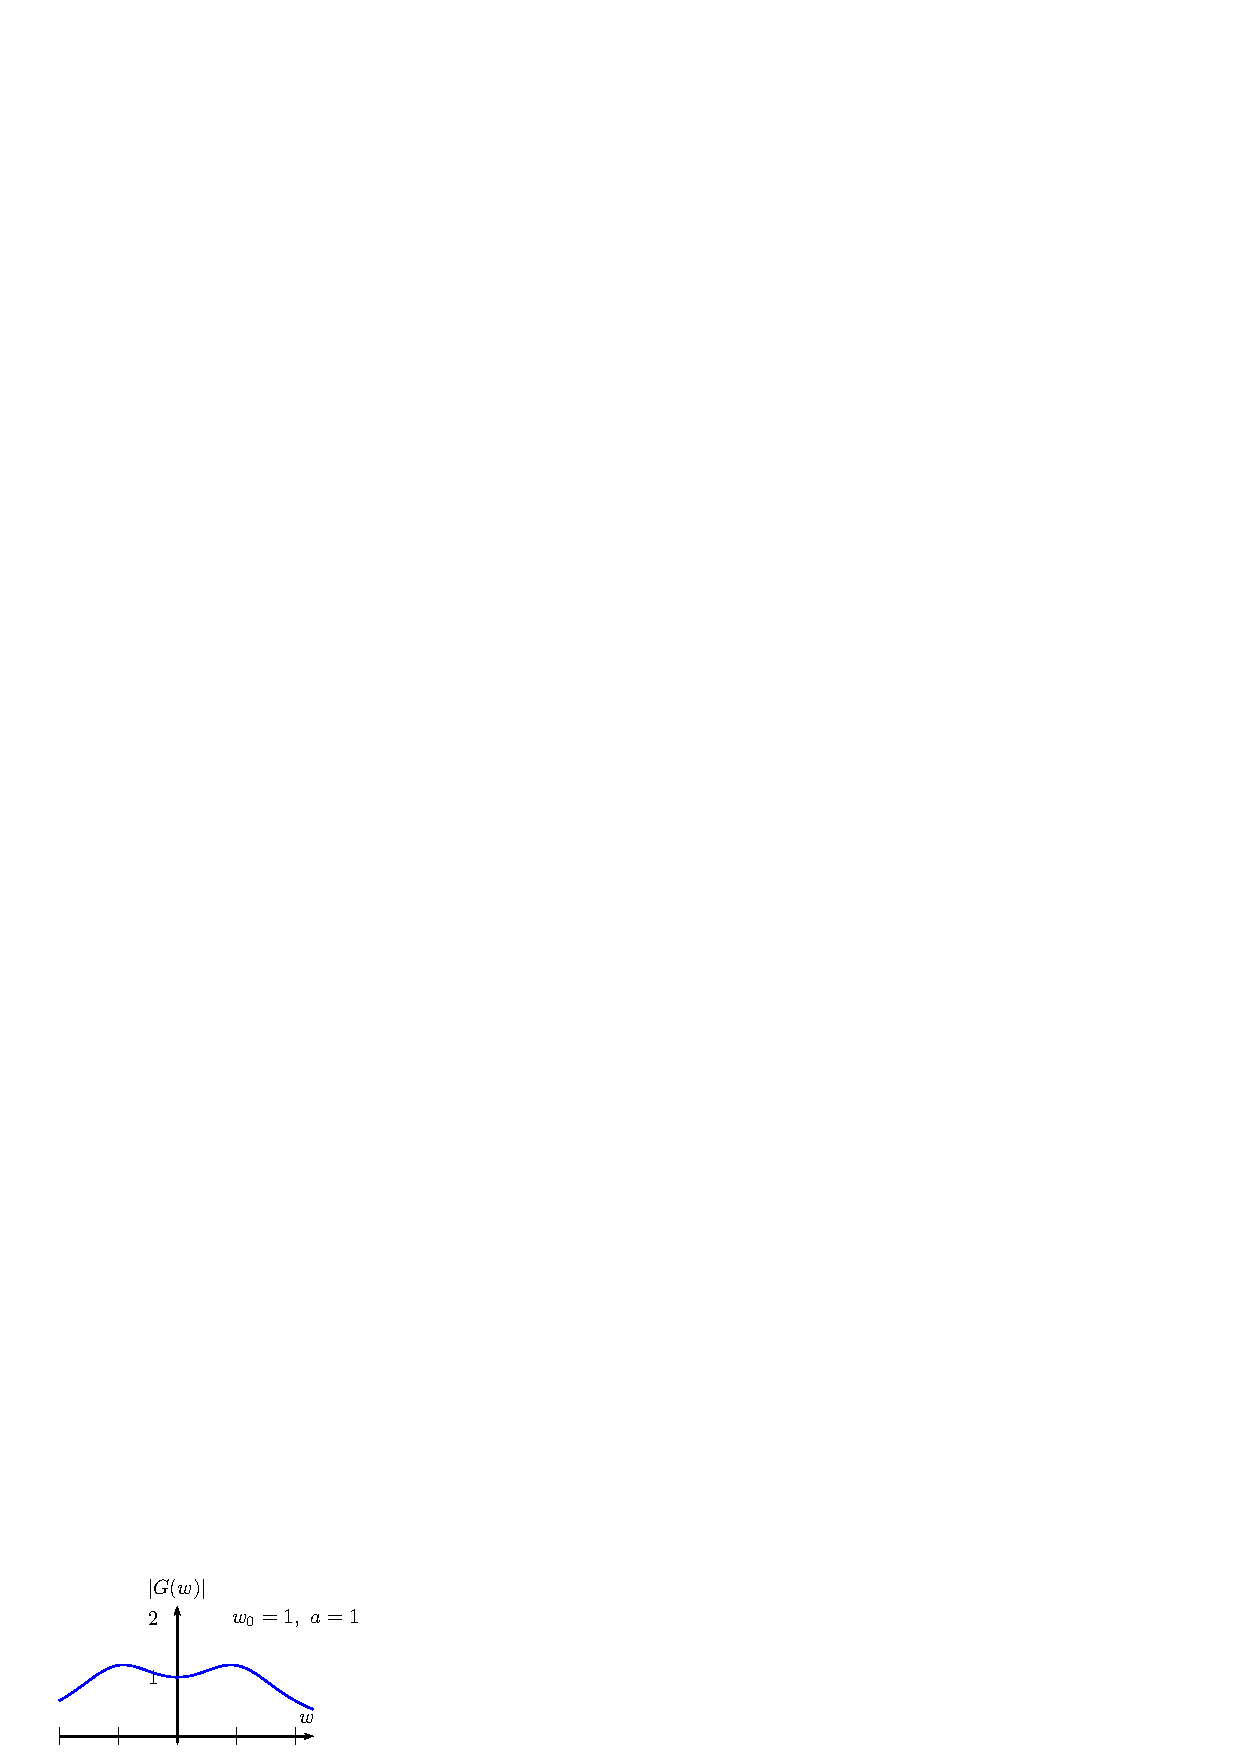
\includegraphics{figs/cap_propriedades_transformada_figura_4}
  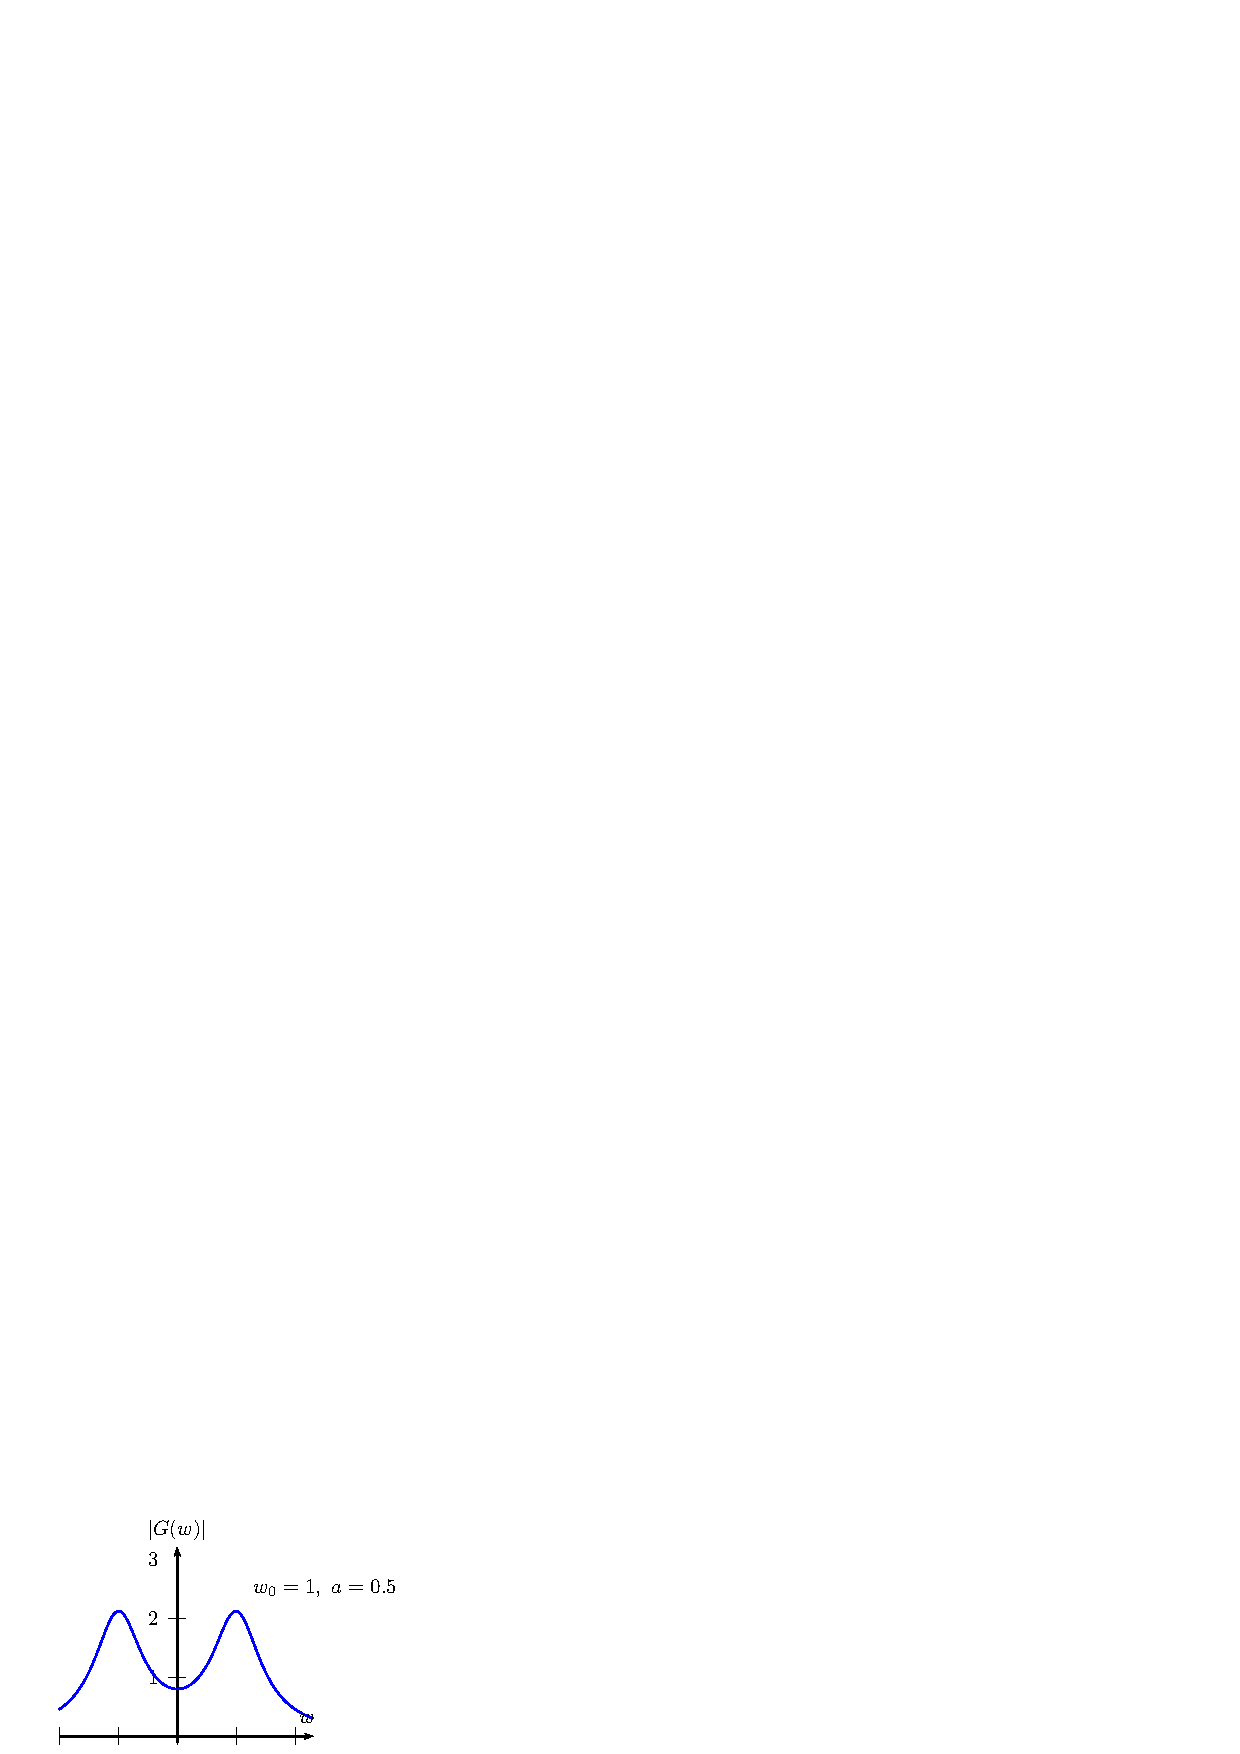
\includegraphics{figs/cap_propriedades_transformada_figura_5}
  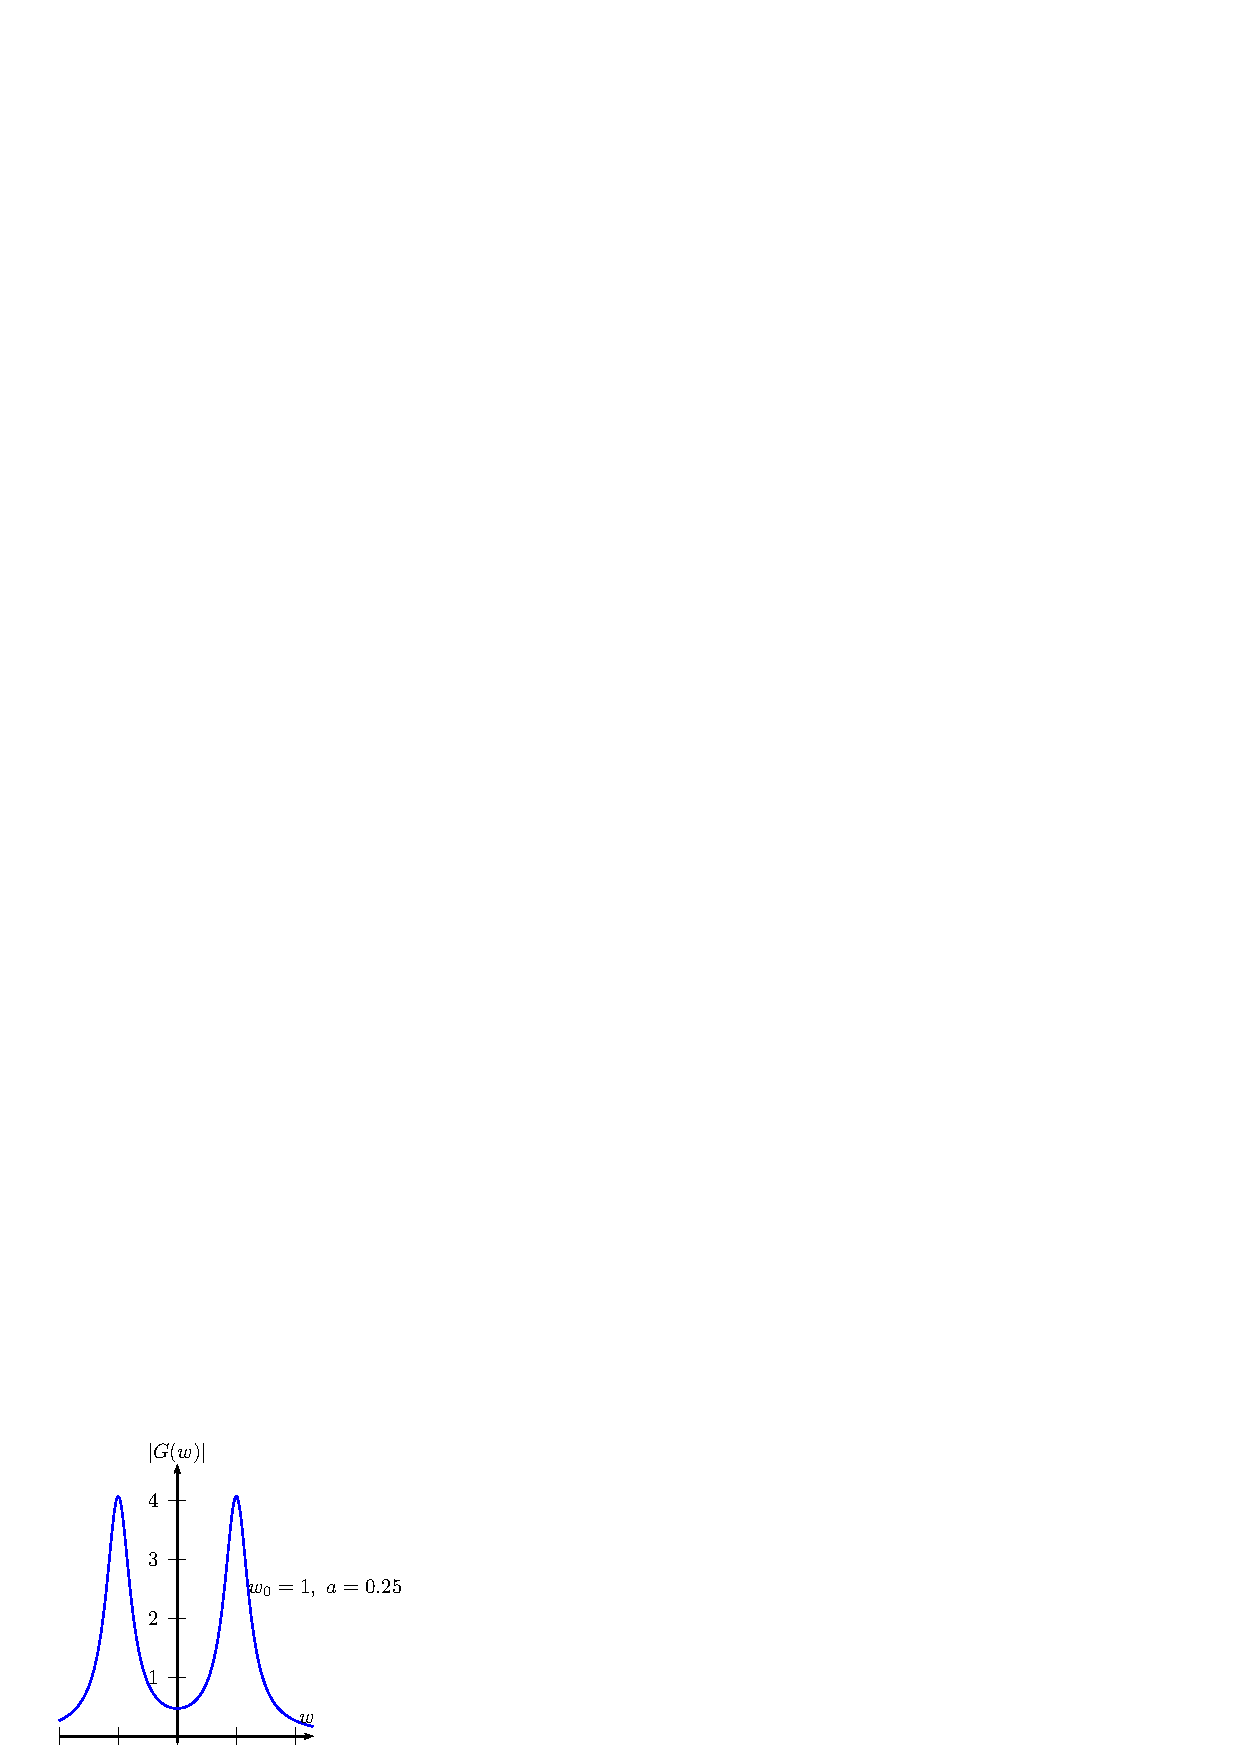
\includegraphics{figs/cap_propriedades_transformada_figura_6}
  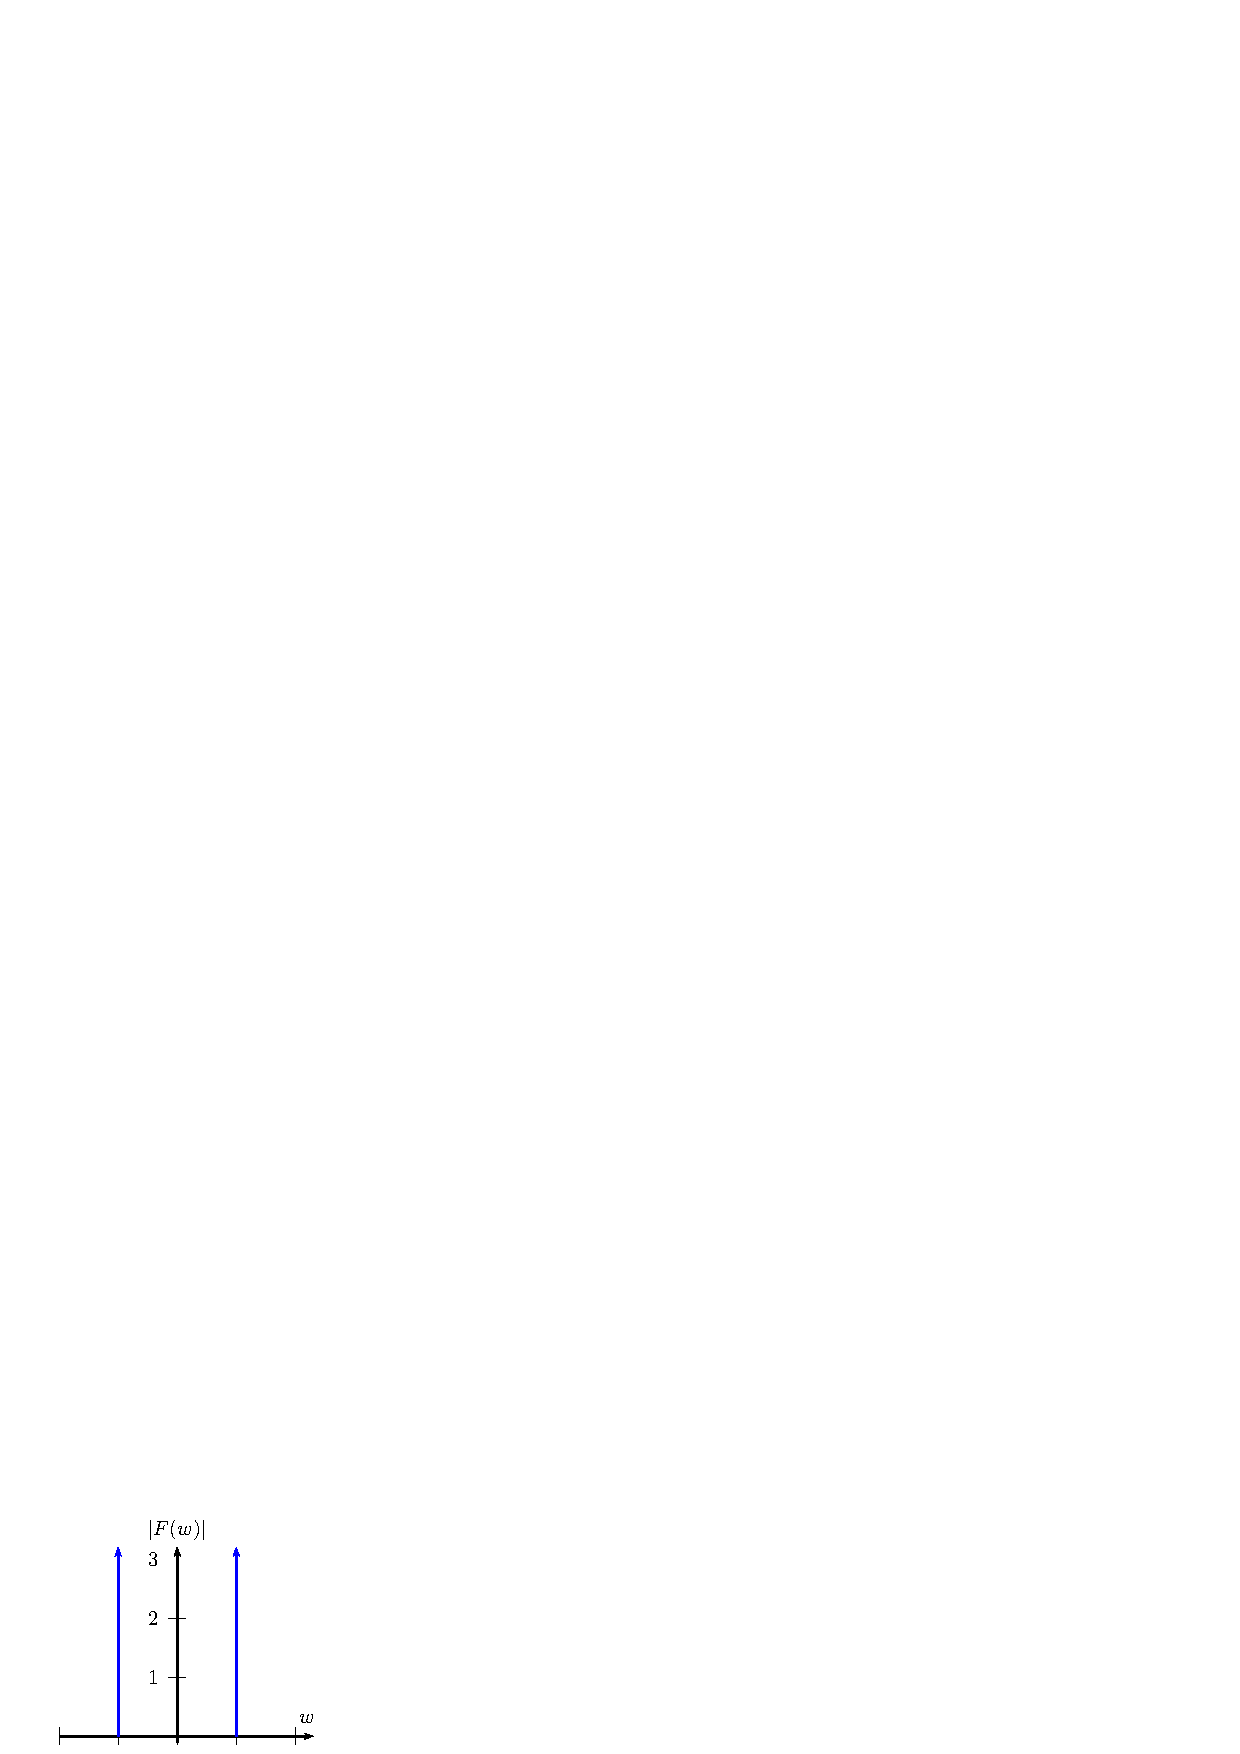
\includegraphics{figs/cap_propriedades_transformada_figura_7}
\end{center}
 \caption{\label{diag_espec_05}}
 \end{figure}
 
% 
% 
 \section{Aplicação: Sinais Discretos}
 Nessa seção vamos discutir sobre discretização de sinais, em especial, pretendemos responder com que frequência precisamos amostrar um sinal real para podermos reconstruí-lo. Vamos considerar que o espectro da função $f(t)$ é composto apenas por frequências inferiores a $w_c$, onde $w_c$ é chamado de frequência de corte. Mostraremos que se conhecermos apenas os valores de $f(t)$ para $t=kT$, $k\in\mathbb{Z}$, onde $T$ é o período de amostragem e $w_a:=\frac{2\pi }{T}>2w_c$  é a frequência de amostragem, então podemos reconstruir exatamente $f(t)$ em todos instantes de tempo.
 Considere $f(t)$ uma função real, definiremos $f_T(t)$ uma versão discretizada deste sinal da seguinte forma:
 \begin{equation}
 f_T(t)=\sum_{k=-\infty}^\infty f(kT) \delta (t-kT),
 \end{equation}
 assim $f_T(t)$ é um trem de Dirac's cujas amplitudes coincidem com o valor da função $f(t)$ nos pontos de amostragem $kT$. Veja um exemplo na figura \ref{sinal_discreto}.
 \begin{figure}[!ht]
 \begin{center}
 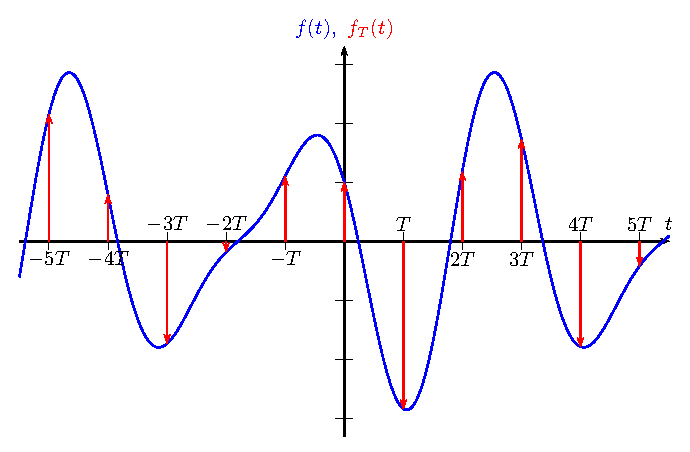
\includegraphics{figs/cap_propriedades_transformada_figura_8}\end{center}
 \caption{\label{sinal_discreto}}
 \end{figure}
 A fim de calcularmos a transforma de Fourier de $f_T(t)$, observamos que:
 \begin{eqnarray*}
 f_T(t)&=&\sum_{k=-\infty}^\infty f(kT) \delta (t-kT)\\
 &=&\sum_{k=-\infty}^\infty f(t) \delta (t-kT)\\
 &=&f(t)\sum_{k=-\infty}^\infty \delta (t-kT)\\
 &=&f(t)\delta_T(t)
 \end{eqnarray*}
 onde $\delta_T(t)=\sum_{k=-\infty}^\infty \delta (t-kT)$ é uma função periódica cuja série de Fourier é dada por:
 \begin{equation}\delta_T(t)=\sum_{k=-\infty}^\infty \delta (t-kT)=\sum_{n=-\infty}^\infty C_n e^{iw_n t}\end{equation}
 e
 \begin{equation}C_n=\frac{1}{T}\int_{-T/2}^{T/2}\delta_T(t) e^{-iw_n t}dt=\frac{1}{T}\end{equation}
 assim,
 \begin{equation}\delta_T(t)=\frac{1}{T}\sum_{n=-\infty}^\infty  e^{iw_n t}\end{equation}
 e, portanto:
 \begin{eqnarray*}
 f_T(t)&=&f(t)\delta_T(t)\\
 &=& f(t)\frac{1}{T}\sum_{n=-\infty}^\infty  e^{iw_n t}\\
 &=&\frac{1}{T}\sum_{n=-\infty}^\infty f(t) e^{iw_n t}
 \end{eqnarray*}
 e finalmente:
 \begin{eqnarray*}
 F_T(w)&=&\mathcal{F}\left\{f_T(t)\right\}\\
 &=&\frac{1}{T}\mathcal{F}\left\{\sum_{n=-\infty}^\infty f(t) e^{iw_n t}\right\}\\
 &=&\frac{1}{T}\sum_{n=-\infty}^\infty F(w-w_n)
 \end{eqnarray*}
 onde se usou a propriedade do deslocamento no eixo $w$ (\ref{prop_desl_w}). Veja um exemplo na figura:
 \begin{figure}[!ht]
 \begin{center}
 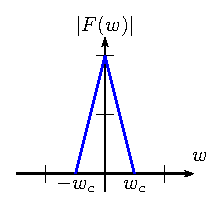
\includegraphics{figs/cap_propriedades_transformada_figura_9}
 \hspace{10pt}
 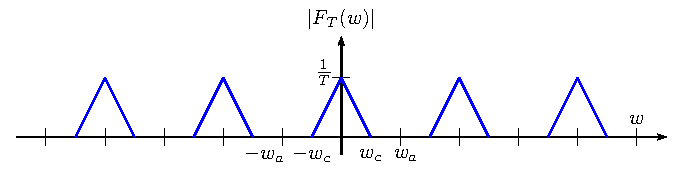
\includegraphics{figs/cap_propriedades_transformada_figura_10}\end{center}
 \caption{\label{sinal_discreto1}}
 \end{figure}
 
 {\bf Obs:} Observamos que se a frequência de amostragem $w_a$ for superior a $2w_c$, então $F_T(w)=\frac{1}{T}F(w)$ no intervalo $[-w_c,w_c]$ e, portanto, toda a informação de $f(t)$ é preservada. De fato, neste caso, podemos escrever:
 \begin{eqnarray*}
 f(t)&=&\frac{1}{2\pi}\int_{-\infty}^\infty F(w)e^{iwt}dw\\
 &=&\frac{1}{2\pi}\int_{-w_c}^{w_c} F(w)e^{iwt}dw\\
 &=&\frac{1}{2\pi}\int_{-w_c}^{w_c} TF_T(w)e^{iwt}dw
 \end{eqnarray*}
% Como $F_T(w)$ pode ser calculada apenas com base nos pontos de amostragem, $f(t)$ pode ser reconstruída. Se $w_a<2w_c$, então existe superposição espectral, o que impede a reconstrução da $f(t)$. Este resultado é conhecido como teorema da amostragem de Nyquist-Shannon ou teorema cardinal da interpolação.
% \end{obs}
% \begin{teo} Suponha que $f(t)$ é uma função real cujo espectro é limitado pela frequência $w_c$, isto é, $F(w)=0$ se $|w|>w_c$, e $T<\frac{\pi}{w_c}$, então
% \begin{equation}
% f(t)=\sum_{n=-\infty}^\infty f(nT) \frac{2\sen\left(\frac{w_a}{2}(t-nT)\right)}{w_a(t-nT)}
% \end{equation}
% \end{teo}
% \begin{proof} Seja $F_T(w)$ a transformada de Fourier do sinal amostrado, conforme vimos, vale a expressão:
% \begin{equation}
% TF_T(w)=\sum_{n=-\infty}^\infty F(w-w_n).
% \end{equation}
% Observe que $TF_T(w)$ é uma função periódica de período $w_a$ (veja figura \ref{sinal_discreto1}), de forma que $TF_T(w)$ admite uma representação em série de Fourier:
% \begin{equation}
% TF_T(w)=\sum_{-\infty}^\infty D_n e^{iv_n w}=\sum_{-\infty}^\infty D_n e^{in Tw},
% \end{equation}
% onde usamos que $v_n=\frac{2\pi n}{w_a}=Tn$ e 
% \begin{eqnarray*}
% D_n&=&\frac{1}{w_a}\int_{-w_a/2}^{w_a/2}TF_T(w)e^{-in Tw}dw\\
% &=&\frac{1}{w_a}\int_{-w_a/2}^{w_a/2}F(w)e^{-in Tw}dw\\
% &=&\frac{1}{w_a}\int_{-\infty}^{\infty}F(w)e^{-in T w}dw,\quad \hbox{pois}\ F(w)=0\ \hbox{se}\ |w|>\frac{w_a}{2}>w_c\\
% &=&\frac{2\pi}{w_a}f(-nT)=Tf(-nT),\quad \hbox{usando a transformada inversa}.
% \end{eqnarray*}
% Logo,
% \begin{equation}
% TF_T(w)=T\sum_{n=-\infty}^\infty f(-nT) e^{in Tw}.
% \end{equation}
% Usando a transformada inversa, temos:
% \begin{eqnarray*}
% f(t)&=&\frac{1}{2\pi}\int_{-w_a/2}^{w_a/2}TF_T(w) e^{i w t}dw\\
% &=&\frac{1}{2\pi}\int_{-w_a/2}^{w_a/2}T\sum_{n=-\infty}^\infty f(-nT) e^{in Tw} e^{i w t}dw\\
% &=&\frac{T}{2\pi}\int_{-w_a/2}^{w_a/2}\sum_{n=-\infty}^\infty f(-nT) e^{iw(t+nT)} dw\\
% &=&\frac{1}{w_a}\sum_{n=-\infty}^\infty f(-nT)\int_{-w_a/2}^{w_a/2}  e^{iw(t+nT)} dw\\
% &=&\frac{1}{w_a}\sum_{n=-\infty}^\infty f(-nT)\int_{-w_a/2}^{w_a/2}  \cos(w(t+nT)) dw,\quad \hbox{pois o seno é ímpar}\\
% &=&\frac{1}{w_a}\sum_{n=-\infty}^\infty f(-nT)\left[  \frac{\sen(w(t+nT))}{t+nT} \right]_{-w_a/2}^{w_a/2}\\
% &=&\sum_{n=-\infty}^\infty f(-nT) \frac{2\sen\left(\frac{w_a}{2}(t+nT)\right)}{w_a(t+nT)} 
% \end{eqnarray*}
% Substituindo $n$ por $-n$ obtemos a expressão:
% \begin{equation}
% f(t)=\sum_{n=-\infty}^\infty f(nT) \frac{2\sen\left(\frac{w_a}{2}(t-nT)\right)}{w_a(t-nT)}.
% \end{equation}
% \end{proof}
% 
% 
% 

 \end{document}
